\begin{filecontents*}[overwrite]{referencias.bib}
@techreport{rfc3535,
  author      = {Schoenwaelder, J.},
  title       = {Overview of the 2002 IAB Network Management Workshop},
  institution = {RFC Editor},
  type        = {RFC},
  number      = {3535},
  year        = {2003},
  doi         = {10.17487/RFC3535},
  url         = {https://www.rfc-editor.org/rfc/rfc3535}
}
@techreport{rfc3411,
  author      = {Harrington, D. and Presuhn, R. and Wijnen, B.},
  title       = {An Architecture for Describing Simple Network Management Protocol (SNMP) Management Frameworks},
  institution = {RFC Editor},
  type        = {RFC},
  number      = {3411},
  year        = {2002},
  doi         = {10.17487/RFC3411},
  url         = {https://www.rfc-editor.org/rfc/rfc3411}
}
@techreport{rfc3416,
  author      = {Presuhn, R.},
  title       = {Version 2 of the Protocol Operations for the Simple Network Management Protocol (SNMP)},
  institution = {RFC Editor},
  type        = {RFC},
  number      = {3416},
  year        = {2002},
  doi         = {10.17487/RFC3416},
  url         = {https://www.rfc-editor.org/rfc/rfc3416}
}
@techreport{rfc6241,
  author      = {Enns, R. and Bjorklund, M. and Schoenwaelder, J. and Bierman, A.},
  title       = {Network Configuration Protocol (NETCONF)},
  institution = {RFC Editor},
  type        = {RFC},
  number      = {6241},
  year        = {2011},
  doi         = {10.17487/RFC6241},
  url         = {https://www.rfc-editor.org/rfc/rfc6241}
}
@techreport{rfc6242,
  author      = {Wasserman, M.},
  title       = {Using the NETCONF Protocol over Secure Shell (SSH)},
  institution = {RFC Editor},
  type        = {RFC},
  number      = {6242},
  year        = {2011},
  doi         = {10.17487/RFC6242},
  url         = {https://www.rfc-editor.org/rfc/rfc6242}
}
@techreport{rfc7950,
  author      = {Bjorklund, M.},
  title       = {The YANG 1.1 Data Modeling Language},
  institution = {RFC Editor},
  type        = {RFC},
  number      = {7950},
  year        = {2016},
  doi         = {10.17487/RFC7950},
  url         = {https://www.rfc-editor.org/rfc/rfc7950}
}
@techreport{rfc7951,
  author      = {Lhotka, L.},
  title       = {JSON Encoding of Data Modeled with YANG},
  institution = {RFC Editor},
  type        = {RFC},
  number      = {7951},
  year        = {2016},
  doi         = {10.17487/RFC7951},
  url         = {https://www.rfc-editor.org/rfc/rfc7951}
}
@techreport{rfc8040,
  author      = {Bierman, A. and Bjorklund, M. and Watsen, K.},
  title       = {RESTCONF Protocol},
  institution = {RFC Editor},
  type        = {RFC},
  number      = {8040},
  year        = {2017},
  doi         = {10.17487/RFC8040},
  url         = {https://www.rfc-editor.org/rfc/rfc8040}
}
@techreport{rfc8343,
  author      = {Bjorklund, M.},
  title       = {A YANG Data Model for Interface Management},
  institution = {RFC Editor},
  type        = {RFC},
  number      = {8343},
  year        = {2018},
  doi         = {10.17487/RFC8343},
  url         = {https://www.rfc-editor.org/rfc/rfc8343}
}
@techreport{rfc8344,
  author      = {Bjorklund, M.},
  title       = {A YANG Data Model for IP Management},
  institution = {RFC Editor},
  type        = {RFC},
  number      = {8344},
  year        = {2018},
  doi         = {10.17487/RFC8344},
  url         = {https://www.rfc-editor.org/rfc/rfc8344}
}
@misc{aws_devops,
  author       = {{Amazon Web Services}},
  title        = {¿Qué es DevOps?},
  year         = {2026},
  howpublished = {\url{https://aws.amazon.com/devops/what-is-devops/}},
  note         = {Consultado el 25 de noviembre de 2026}
}
@misc{cisco_devops,
  author       = {{Cisco Systems, Inc.}},
  title        = {What is DevOps?},
  year         = {2026},
  howpublished = {\url{https://www.cisco.com/c/en/us/solutions/cloud/what-is-devops.html}},
  note         = {Consultado el 25 de noviembre de 2026}
}
@misc{pyang,
  author       = {{Pyang Project}},
  title        = {Pyang: A YANG validator and converter},
  year         = {2026},
  howpublished = {\url{https://github.com/mbj4668/pyang}},
  note         = {Consultado el 25 de noviembre de 2026}
}
@misc{yangmodels,
  author       = {{YangModels}},
  title        = {Repositorio público de módulos YANG estándar},
  year         = {2026},
  howpublished = {\url{https://github.com/YangModels/yang}},
  note         = {Consultado el 25 de noviembre de 2026}
}
@misc{postman,
  author       = {{Postman, Inc.}},
  title        = {Send a request with the Postman API client},
  year         = {2026},
  howpublished = {\url{https://learning.postman.com/docs/use/send-requests/create-requests/request-basics/}},
  note         = {Documentación oficial}
}
@misc{postman_req,
  author       = {{Postman, Inc.}},
  title        = {Postman system requirements},
  year         = {2026},
  howpublished = {\url{https://learning.postman.com/docs/getting-started/installation/system-requirements}},
  note         = {Consultado el 25 de noviembre de 2026}
}
@misc{ansible,
  author       = {{Red Hat Ansible}},
  title        = {Ansible Network Automation},
  year         = {2026},
  howpublished = {\url{https://docs.ansible.com/ansible/latest/network/}},
  note         = {Documentación oficial}
}
@misc{ansible_install,
  author       = {{Red Hat Ansible}},
  title        = {Installation Guide: Control node and managed node requirements},
  year         = {2026},
  howpublished = {\url{https://docs.ansible.com/ansible/latest/installation_guide/intro_installation.html}},
  note         = {Consultado el 25 de noviembre de 2026}
}
@misc{nornir,
  author       = {{Nornir Project}},
  title        = {Nornir Documentation},
  year         = {2026},
  howpublished = {\url{https://nornir.readthedocs.io/}},
  note         = {Consultado el 25 de noviembre de 2026}
}
@misc{salt,
  author       = {{Salt Project}},
  title        = {Salt overview},
  year         = {2026},
  howpublished = {\url{https://docs.saltproject.io/salt/user-guide/en/latest/topics/overview.html}},
  note         = {Consultado el 25 de noviembre de 2026}
}
@misc{salt_arch,
  author       = {{Salt Project}},
  title        = {Salt system architecture},
  year         = {2026},
  howpublished = {\url{https://docs.saltproject.io/en/3006/topics/salt_system_architecture.html}},
  note         = {Consultado el 25 de noviembre de 2026}
}
@misc{salt_os,
  author       = {{Salt Project}},
  title        = {Salt supported operating systems},
  year         = {2026},
  howpublished = {\url{https://docs.saltproject.io/salt/install-guide/en/latest/topics/salt-supported-operating-systems.html}},
  note         = {Consultado el 25 de noviembre de 2026}
}
@misc{cisco_restconf,
  author       = {{Cisco Systems, Inc.}},
  title        = {Explore and learn about open management interfaces},
  year         = {2026},
  howpublished = {\url{https://developer.cisco.com/site/standard-network-devices/}},
  note         = {Tabla de soporte de NETCONF y RESTCONF por plataforma. Consultado el 25 de noviembre de 2026}
}
@misc{pt_controller,
  author       = {{Cisco Networking Academy}},
  title        = {Configuring Network Controllers -- Cisco Packet Tracer Help},
  year         = {2026},
  howpublished = {\url{https://tutorials.ptnetacad.net/help/default/config_NetworkControllers.htm}},
  note         = {Consultado el 25 de noviembre de 2026}
}
@misc{devnet_sandbox,
  author       = {{Cisco DevNet}},
  title        = {Cisco IOS XE Sandboxes},
  year         = {2026},
  howpublished = {\url{https://developer.cisco.com/docs/ios-xe-voip/sandbox}},
  note         = {Consultado el 25 de noviembre de 2026}
}
@misc{repositorio,
  author       = {{Equipo del proyecto}},
  title        = {Proyecto\_Redes: administración de interfaces mediante YANG, RESTCONF y Python},
  year         = {2026},
  howpublished = {\url{https://github.com/CAMF0712/Proyecto_Redes}},
  note         = {Repositorio del código, laboratorio y evidencias}
}
@misc{devnet_faq,
  author       = {{Cisco DevNet}},
  title        = {DevNet Sandbox FAQs: cost, access, and troubleshooting},
  year         = {2026},
  howpublished = {\url{https://developer.cisco.com/docs/sandbox/faqs}},
  note         = {Consultado el 25 de noviembre de 2026}
}
\end{filecontents*}

\documentclass[12pt,letterpaper]{article}

% Compilar con pdfLaTeX + Biber (por ejemplo, en Overleaf). Las figuras están
% en la carpeta figuras/ junto a este archivo.
\usepackage[utf8]{inputenc}
\usepackage[T1]{fontenc}
\usepackage[spanish,es-nodecimaldot,es-noshorthands,es-tabla]{babel}
\usepackage[scaled=0.95]{helvet}
\renewcommand{\familydefault}{\sfdefault}
\usepackage{microtype}
\usepackage{geometry}
\geometry{letterpaper, left=2.5cm, right=2.5cm, top=2.5cm, bottom=2.5cm}
\usepackage{setspace}
\onehalfspacing
\usepackage{ragged2e}
\usepackage{graphicx}
\graphicspath{{figuras/}}
\usepackage{float}
\usepackage{booktabs}
\usepackage{tabularx}
\usepackage{longtable}
\usepackage{array}
\usepackage{enumitem}
\usepackage{xcolor}
\usepackage{listings}
\usepackage{caption}
\usepackage{titlesec}
\usepackage{xurl}
\usepackage{hyperref}
\usepackage{csquotes}
\usepackage[style=apa,backend=biber,sortcites=true]{biblatex}
\DeclareLanguageMapping{spanish}{spanish-apa}
\addbibresource{referencias.bib}

\hypersetup{
  colorlinks=true,
  linkcolor=black,
  citecolor=black,
  urlcolor=blue,
  pdftitle={Desafío de Redes: Programabilidad basada en modelos},
  pdfauthor={Vega, Loría, Mora, Villatoro, Rojas}
}

% La consigna solicita Arial 12. Se utiliza Helvetica como sustituto tipográfico
% compatible y disponible en Overleaf. Si se dispone de Arial, puede cambiarse
% la familia mediante fontspec al compilar con XeLaTeX.
\titleformat{\section}{\normalfont\bfseries\fontsize{12}{14}\selectfont}{\thesection}{0.7em}{}
\titleformat{\subsection}{\normalfont\bfseries\fontsize{12}{14}\selectfont}{\thesubsection}{0.7em}{}
\titleformat{\subsubsection}{\normalfont\bfseries\fontsize{12}{14}\selectfont}{\thesubsubsection}{0.7em}{}
\setlength{\parindent}{1.25cm}
\setlength{\parskip}{0.15cm}
\captionsetup{font=small,labelfont=bf,textfont=normalfont,justification=centering}
\renewcommand{\lstlistingname}{Listado}
\renewcommand{\lstlistlistingname}{Índice de listados}

\definecolor{codebg}{RGB}{245,245,245}
\definecolor{codeframe}{RGB}{210,210,210}
\lstdefinestyle{codigo}{
  backgroundcolor=\color{codebg},
  basicstyle=\ttfamily\footnotesize,
  frame=single,
  rulecolor=\color{codeframe},
  breaklines=true,
  columns=fullflexible,
  keepspaces=true,
  showstringspaces=false,
  tabsize=2,
  literate={á}{{\'a}}1 {é}{{\'e}}1 {í}{{\'i}}1 {ó}{{\'o}}1 {ú}{{\'u}}1
           {Á}{{\'A}}1 {É}{{\'E}}1 {Í}{{\'I}}1 {Ó}{{\'O}}1 {Ú}{{\'U}}1
           {ñ}{{\~n}}1 {Ñ}{{\~N}}1 {¿}{{?`}}1 {¡}{{!`}}1
}
\lstset{style=codigo}

\newcommand{\pendiente}[1]{\textcolor{red}{\textbf{[PENDIENTE: #1]}}}

\begin{document}
\justifying
\setlength{\emergencystretch}{3em}

% ----------------------------------------------------------------------
% PORTADA
% ----------------------------------------------------------------------
\begin{titlepage}
  \centering
  {\large INSTITUTO TECNOLÓGICO DE COSTA RICA\par}
  {\large ESCUELA DE INGENIERÍA EN COMPUTADORES\par}
  \vspace{1.2cm}
  {\large CE-5301 REDES DE COMPUTADORAS\par}
  \vspace{1.6cm}
  {\LARGE\bfseries TRABAJO FINAL: DESAFÍO DE REDES\par}
  \vspace{0.7cm}
  {\Large Programabilidad de redes basada en modelos mediante YANG y RESTCONF\par}
  \vspace{1.4cm}
  {\large\bfseries Integrantes:\par}
  \vspace{0.3cm}
  \begin{tabular}{ll}
    Giancarlo Vega Marín & 2020195338 \\
    José Manuel Loría Cordero & 2022211671 \\
    César Andrés Mora Fajardo & 2020053458 \\
    Marco Villatoro Chacon & 2021057692 \\
    Mariana Rojas Rojas & 2020076936 \\
  \end{tabular}\par
  \vfill
  \begin{flushleft}
    \textbf{Profesor:} Rodolfo Tacsan Chaves\\
    \textbf{Periodo:} II semestre de 2026\\
    \textbf{Fecha de entrega:} 26 de noviembre, 2026
  \end{flushleft}
  \vspace{1cm}
  {Cartago, Costa Rica\par}
\end{titlepage}

\tableofcontents
\newpage

% ----------------------------------------------------------------------
% OBJETIVOS
% ----------------------------------------------------------------------
\section{Objetivos del desafío}

\subsection{Objetivo general de la investigación}
Investigar los fundamentos de la programabilidad de redes basada en modelos, el modelado de datos mediante YANG y los mecanismos NETCONF y RESTCONF, con el propósito de comprender su aplicación en la administración moderna de infraestructuras de red.

\subsection{Objetivos específicos de la investigación}
\begin{enumerate}[label=\arabic*.]
  \item Explicar el propósito y los fundamentos de la programabilidad de redes basada en modelos, incluyendo el papel de DevOps, SNMP y el RFC 3535.
  \item Describir el lenguaje YANG, sus modelos de datos, la estructura de sus elementos y el uso de herramientas como Pyang.
  \item Analizar el funcionamiento de NETCONF, sus operaciones, transporte, mensajes RPC y relación con YANG.
  \item Analizar RESTCONF, su relación con YANG y sus diferencias respecto a NETCONF.
  \item Investigar el uso de Postman y Python para construir y ejecutar solicitudes API REST.
  \item Comparar al menos tres herramientas de automatización de redes según su método de operación, arquitectura de gestión y sistemas operativos compatibles.
\end{enumerate}

\subsection{Objetivo general del caso de uso}
Diseñar y evaluar una solución de administración de interfaces de red mediante una aplicación en Python que utilice una API RESTCONF y modelos YANG para consultar información y realizar modificaciones controladas sobre un dispositivo compatible o, cuando el entorno disponible no lo permita, sobre un simulador local claramente identificado.

\subsection{Objetivos específicos del caso de uso}
\begin{enumerate}[label=\arabic*.]
  \item Construir una topología de laboratorio en Cisco Packet Tracer para representar la infraestructura de red y verificar configuraciones y conectividad mediante CLI.
  \item Desarrollar una aplicación que permita consultar interfaces, visualizar sus propiedades y registrar las operaciones realizadas.
  \item Implementar y probar solicitudes GET y PATCH/PUT mediante RESTCONF en un entorno compatible o simulado, diferenciando explícitamente ambos escenarios.
  \item Verificar los cambios realizados mediante consultas posteriores y analizar las respuestas HTTP obtenidas.
\end{enumerate}

% ----------------------------------------------------------------------
% INVESTIGACION
% ----------------------------------------------------------------------
\section{Investigación}

\subsection{Programabilidad de redes basada en modelos}

\subsubsection{Definición y propósito}
La programabilidad de redes basada en modelos es un enfoque de administración en el que la información de configuración y de estado de los dispositivos se representa mediante modelos de datos estructurados. Estos modelos permiten que las aplicaciones conozcan de antemano la organización de los datos y puedan consultarlos o modificarlos mediante interfaces programables. En lugar de depender de comandos de texto propios de cada fabricante, cuyo formato de salida puede cambiar entre versiones, las aplicaciones intercambian información estructurada con los dispositivos administrados. Los modelos YANG se utilizan con protocolos como NETCONF y RESTCONF para describir y transportar estos datos \parencite{rfc7950,rfc6241,rfc8040}.

Este enfoque resulta relevante cuando una infraestructura requiere cambios repetitivos, consistencia entre equipos, validación de parámetros e integración con sistemas externos. La automatización no elimina la necesidad de diseñar, controlar y verificar los cambios; proporciona mecanismos para ejecutarlos de manera sistemática y reproducible.

\subsubsection{¿Qué hace un equipo DevOps?}
DevOps es una combinación de filosofía cultural, prácticas y herramientas cuyo objetivo es aumentar la capacidad de una organización para entregar aplicaciones y servicios con rapidez y confiabilidad. Bajo este modelo, los equipos de desarrollo y de operaciones dejan de trabajar aislados y colaboran durante todo el ciclo de vida del servicio, desde el desarrollo y las pruebas hasta el despliegue y la operación \parencite{aws_devops}. Cisco lo describe como una filosofía que integra a los equipos de desarrollo y de operaciones de TI para que colaboren a lo largo del ciclo de vida del software, lo que exige un cambio cultural basado en mayor comunicación entre equipos \parencite{cisco_devops}.

Entre las prácticas habituales de un equipo DevOps se encuentran la integración y la entrega continuas, la infraestructura como código, la gestión de configuración mediante código, el control de versiones, las pruebas automatizadas y el monitoreo continuo \parencite{aws_devops}. Aplicadas a redes (enfoque a menudo llamado \textit{NetDevOps}), estas prácticas implican mantener las configuraciones y los scripts en un repositorio, revisar los cambios antes de aplicarlos, probarlos en un entorno controlado, desplegarlos de forma automatizada y verificar el resultado. El presente proyecto sigue ese esquema a pequeña escala: el código, las configuraciones del laboratorio y las pruebas se versionan en un repositorio Git, y cada cambio de configuración se confirma y se verifica de forma automática.

\subsubsection{Rol de SNMP}
SNMP (\textit{Simple Network Management Protocol}) es el protocolo tradicional de supervisión y administración de dispositivos de red. Su arquitectura, descrita en el RFC 3411, distingue entre entidades SNMP que actúan como \textit{administradores} (aplicaciones que generan comandos y reciben notificaciones) y como \textit{agentes} (que responden a comandos y emiten notificaciones). La información administrable se organiza en bases de información de gestión (MIB) y cada variable se identifica mediante un identificador de objeto (OID). La misma arquitectura introduce SNMPv3 con un modelo de seguridad basado en usuarios que añade autenticación y privacidad \parencite{rfc3411}.

Las operaciones de SNMPv2, definidas en el RFC 3416, incluyen \texttt{GetRequest}, \texttt{GetNextRequest} y \texttt{GetBulkRequest} para leer variables, \texttt{SetRequest} para modificarlas, \texttt{Response} como respuesta del agente, y \texttt{SNMPv2-Trap} e \texttt{InformRequest} para notificaciones asíncronas \parencite{rfc3416}.

En la práctica, SNMP se ha utilizado sobre todo para el monitoreo: disponibilidad, contadores de tráfico y estado de interfaces. El taller del IAB documentado en el RFC 3535 constató que los operadores rara vez usaban SNMP para configurar equipos y preferían la CLI, lo que motivó el desarrollo de nuevos mecanismos de configuración \parencite{rfc3535}. Por ello, SNMP y NETCONF/RESTCONF suelen coexistir: el primero para supervisión y los segundos para la administración de la configuración mediante modelos YANG.

\subsubsection{¿Qué es el RFC 3535?}
El RFC 3535 resume el taller de administración de redes organizado por el IAB (\textit{Internet Architecture Board}) en junio de 2002, en el que operadores y desarrolladores de protocolos analizaron por qué las herramientas estándar no satisfacían las necesidades de configuración. Entre sus observaciones destacan las siguientes \parencite{rfc3535}:
\begin{itemize}
  \item SNMP funciona razonablemente para el monitoreo, pero se usa poco para la configuración.
  \item Los operadores necesitan distinguir claramente los datos de configuración de los datos operativos y de estado.
  \item Se requiere poder configurar la red como un todo, con transacciones que involucren varios dispositivos y con la posibilidad de revertir cambios.
  \item Las configuraciones deberían poder exportarse, compararse y almacenarse como texto, aprovechando herramientas existentes de control de versiones.
  \item Es deseable un lenguaje de modelado de datos legible por personas y que permita validar los datos.
\end{itemize}
Estas recomendaciones son el antecedente directo de NETCONF y, posteriormente, del lenguaje YANG y de RESTCONF.

\subsubsection{Bloques básicos de construcción}
En una solución de programabilidad basada en modelos pueden identificarse los siguientes componentes:
\begin{itemize}
  \item \textbf{Modelo de datos:} define la estructura y las restricciones de la información.
  \item \textbf{Lenguaje de modelado:} permite describir formalmente los datos; YANG es el lenguaje utilizado en redes.
  \item \textbf{Codificación:} representa las instancias de datos para el transporte, por ejemplo XML o JSON \parencite{rfc7951}.
  \item \textbf{Protocolo de administración:} permite intercambiar datos y ejecutar operaciones; NETCONF y RESTCONF son ejemplos.
  \item \textbf{Aplicación cliente o sistema administrador:} construye solicitudes, autentica, procesa respuestas y controla operaciones.
  \item \textbf{Dispositivo administrado:} implementa los modelos y expone los servicios de administración.
\end{itemize}

\subsubsection{¿Qué es un modelo de datos?}
Un modelo de datos es una descripción formal de la estructura, los tipos, las relaciones y las restricciones de la información que administra un sistema. En redes puede representar interfaces, direcciones IP, protocolos de enrutamiento, parámetros de seguridad y estados operativos. El modelo permite que el cliente y el dispositivo interpreten los datos según una estructura común y que los datos se validen antes de aplicarse.

\subsection{Introducción al modelo YANG}

\subsubsection{¿Qué es YANG?}
YANG (\textit{Yet Another Next Generation}) es un lenguaje de modelado de datos utilizado para describir datos de configuración, datos de estado, operaciones RPC y notificaciones de los protocolos de administración de red. La versión 1.1 se especifica en el RFC 7950 \parencite{rfc7950}. YANG define la estructura de los datos, pero no es por sí mismo el protocolo que los transporta.

\subsubsection{Lenguaje YANG, modelos YANG y datos YANG}
\begin{description}[style=nextline]
  \item[Lenguaje YANG] Conjunto de reglas y construcciones sintácticas para definir modelos.
  \item[Modelo o módulo YANG] Definición concreta escrita con el lenguaje; por ejemplo, el módulo \texttt{ietf-interfaces} describe las interfaces de un dispositivo \parencite{rfc8343}.
  \item[Datos YANG] Instancias de información que siguen la estructura definida por uno o más modelos, codificadas en XML o JSON.
\end{description}

\subsubsection{Estructura de un modelo YANG}
Entre las construcciones habituales se encuentran \texttt{module}, \texttt{namespace}, \texttt{prefix}, \texttt{import}, \texttt{container}, \texttt{list}, \texttt{leaf}, \texttt{leaf-list}, \texttt{typedef}, \texttt{identity}, \texttt{augment} y \texttt{description}. Los contenedores agrupan nodos; las listas representan colecciones de elementos identificados por claves; las hojas contienen valores individuales; \texttt{augment} permite que un módulo agregue nodos a otro. Las hojas pueden marcarse como de configuración (\texttt{config true}) o de solo lectura (\texttt{config false}) \parencite{rfc7950}.

El Listado~\ref{lst:yang} muestra un módulo simplificado con fines ilustrativos.
\begin{lstlisting}[language={},caption={Fragmento ilustrativo de un modelo YANG},label={lst:yang}]
module ejemplo-interfaces {
  yang-version 1.1;
  namespace "urn:ejemplo:interfaces";
  prefix "ifx";

  container interfaces {
    list interface {
      key "name";
      leaf name { type string; }
      leaf description { type string; }
      leaf enabled { type boolean; default true; }
    }
  }
}
\end{lstlisting}

En el proyecto se utilizaron los módulos estándar \texttt{ietf-interfaces} (RFC 8343) e \texttt{ietf-ip} (RFC 8344). El segundo usa \texttt{augment} para agregar a cada interfaz el contenedor \texttt{ipv4} con su lista de direcciones, cuya subred se expresa mediante \texttt{prefix-length} o \texttt{netmask} \parencite{rfc8343,rfc8344}.

\subsubsection{¿Qué es Pyang y cómo se utiliza?}
Pyang es una herramienta de línea de comandos, escrita en Python, para validar módulos YANG y convertirlos a otros formatos, entre ellos una vista en árbol de la jerarquía de nodos \parencite{pyang}. Los módulos del proyecto se descargaron del repositorio público YangModels \parencite{yangmodels} y se validaron con pyang 2.7.1 en modo estricto, sin errores ni advertencias. El Listado~\ref{lst:pyang} muestra los comandos y un extracto real del árbol generado.

\begin{lstlisting}[language=bash,caption={Validación y vista en árbol de los modelos del proyecto (extracto)},label={lst:pyang}]
pip install pyang
pyang -p models --strict models/ietf-interfaces.yang models/ietf-ip.yang
pyang -p models -f tree models/ietf-interfaces.yang models/ietf-ip.yang

module: ietf-interfaces
  +--rw interfaces
  |  +--rw interface* [name]
  |     +--rw name                        string
  |     +--rw description?                string
  |     +--rw type                        identityref
  |     +--rw enabled?                    boolean
  |     +--ro admin-status                enumeration {if-mib}?
  |     +--ro oper-status                 enumeration
  |     +--rw ip:ipv4!
  |     |  +--rw ip:address* [ip]
  |     |  |  +--rw ip:ip                     inet:ipv4-address-no-zone
  |     |  |  +--rw (ip:subnet)
  |     |  |  |  +--:(ip:prefix-length)
  |     |  |  |  |  +--rw ip:prefix-length?   uint8
  |     |  |  |  +--:(ip:netmask)
  |     |  |  |     +--rw ip:netmask?         yang:dotted-quad
  x--ro interfaces-state
\end{lstlisting}

En el árbol, \texttt{rw} indica datos de configuración, \texttt{ro} datos de estado, \texttt{*} una lista, \texttt{?} un nodo opcional y \texttt{x} un nodo obsoleto (\textit{deprecated}): en el RFC 8343 el estado operativo se trasladó a \texttt{/interfaces} y \texttt{interfaces-state} se conserva solo por compatibilidad \parencite{rfc8343}.

\subsection{Exploración de YANG mediante NETCONF}

\subsubsection{¿Qué es NETCONF y bajo qué estándar fue creado?}
NETCONF (\textit{Network Configuration Protocol}) es un protocolo de administración de red desarrollado por el IETF. Su versión actual se define en el RFC 6241, que reemplaza al RFC 4741 original. Permite instalar, manipular y eliminar la configuración de los dispositivos mediante operaciones estructuradas entre un cliente y un servidor NETCONF \parencite{rfc6241}.

\subsubsection{Funcionamiento de la comunicación}
NETCONF se organiza conceptualmente en cuatro capas: contenido (los datos de configuración y estado, modelados en YANG), operaciones (\texttt{<get-config>}, \texttt{<edit-config>}, etc.), mensajes (\texttt{<rpc>} y \texttt{<rpc-reply>}) y transporte seguro \parencite{rfc6241}. Al iniciar una sesión, cliente y servidor intercambian mensajes \texttt{<hello>} con sus capacidades, por ejemplo el soporte de un datastore \textit{candidate} o de confirmación de cambios. El transporte obligatorio es SSH, sobre el puerto TCP 830 asignado para este fin \parencite{rfc6242}. NETCONF distingue datastores de configuración: \texttt{running} (configuración activa) y, según las capacidades, \texttt{candidate} y \texttt{startup}.

\subsubsection{Operaciones y ejemplo de llamada}
Las operaciones base de NETCONF son \texttt{<get>}, \texttt{<get-config>}, \texttt{<edit-config>}, \texttt{<copy-config>}, \texttt{<delete-config>}, \texttt{<lock>}, \texttt{<unlock>}, \texttt{<close-session>} y \texttt{<kill-session>}; capacidades opcionales añaden \texttt{<commit>}, \texttt{<discard-changes>} y \texttt{<validate>} \parencite{rfc6241}. El Listado~\ref{lst:netconf} solicita la configuración del datastore \texttt{running}.

\begin{lstlisting}[language=XML,caption={Ejemplo de solicitud NETCONF get-config},label={lst:netconf}]
<rpc message-id="101"
     xmlns="urn:ietf:params:xml:ns:netconf:base:1.0">
  <get-config>
    <source><running/></source>
  </get-config>
</rpc>
\end{lstlisting}

\subsubsection{¿Qué es una RPC y qué formato utiliza?}
Una RPC (\textit{Remote Procedure Call}) es una solicitud para que un sistema remoto ejecute una operación y devuelva un resultado. En NETCONF, cada solicitud se envía dentro de un elemento XML \texttt{<rpc>} identificado por un atributo \texttt{message-id}, y el servidor responde con un \texttt{<rpc-reply>} con el mismo identificador, que contiene los datos solicitados, un \texttt{<ok/>} o elementos \texttt{<rpc-error>} \parencite{rfc6241}.

\subsection{Exploración de YANG mediante RESTCONF}

\subsubsection{¿Qué es RESTCONF?}
RESTCONF es un protocolo basado en HTTP que ofrece una interfaz programática para acceder a datos definidos en YANG, usando los conceptos de datastores de NETCONF. Su especificación es el RFC 8040. Los datos se exponen como recursos bajo una raíz (normalmente \texttt{/restconf}) y se representan en XML o JSON con los tipos de medio \texttt{application/yang-data+xml} y \texttt{application/yang-data+json} \parencite{rfc8040,rfc7951}.

\begin{table}[H]
\centering
\caption{Métodos HTTP en RESTCONF \parencite{rfc8040}}
\begin{tabularx}{\textwidth}{p{2.2cm}X}
\toprule
\textbf{Método} & \textbf{Uso} \\
\midrule
GET & Recuperar datos de configuración o de estado de un recurso \\
POST & Crear un recurso hijo o invocar una operación \\
PUT & Crear o reemplazar por completo el recurso indicado \\
PATCH & Combinar (\textit{merge}) el cuerpo con el recurso existente \\
DELETE & Eliminar el recurso \\
\bottomrule
\end{tabularx}
\end{table}

\subsubsection{Diferencias entre NETCONF y RESTCONF}
\begin{table}[H]
\centering
\caption{Comparación general entre NETCONF y RESTCONF}
\begin{tabularx}{\textwidth}{>{\bfseries}p{3cm}XX}
\toprule
Característica & NETCONF & RESTCONF \\
\midrule
Interfaz & Operaciones RPC & Recursos accesibles mediante métodos HTTP \\
Transporte & SSH obligatorio (puerto 830) & HTTPS \\
Formato & XML & XML o JSON \\
Modelo & YANG & YANG \\
Sesión & Con estado; intercambio de capacidades & Sin estado; cada solicitud es independiente \\
Transacciones & Datastore \textit{candidate}, \texttt{lock}, \texttt{commit} & Cada solicitud se aplica de forma individual \\
\bottomrule
\end{tabularx}
\end{table}

La ventaja práctica de RESTCONF para este proyecto es que utiliza mecanismos HTTP conocidos por herramientas de desarrollo y clientes API, lo que facilita las pruebas con Postman y la integración con bibliotecas HTTP de Python. Esto no implica que RESTCONF sea superior a NETCONF; la elección depende de las capacidades del equipo y de requisitos como las transacciones entre varios dispositivos \parencite{rfc6241,rfc8040}.

\subsubsection{Relación entre YANG y las llamadas RESTCONF}
YANG define la estructura de los datos y RESTCONF construye las URL a partir de esa estructura: el nombre del módulo y del nodo forman la ruta, y las claves de las listas se indican con \texttt{=}. Por ejemplo, la interfaz \texttt{GigabitEthernet0/0/1} de la lista \texttt{interface} se identifica como \texttt{interface=GigabitEthernet0\%2F0\%2F1}, porque los caracteres reservados de la clave deben codificarse \parencite{rfc8040}. La ruta exacta, los nodos disponibles y los métodos aceptados dependen de los modelos que implemente el dispositivo.

\begin{lstlisting}[language={},caption={Endpoints RESTCONF utilizados en el proyecto}]
GET   /restconf/data/ietf-interfaces:interfaces
GET   /restconf/data/ietf-interfaces:interfaces/interface=GigabitEthernet0%2F0%2F1
PATCH /restconf/data/ietf-interfaces:interfaces/interface=GigabitEthernet0%2F0%2F1
PUT   /restconf/data/ietf-interfaces:interfaces/interface=GigabitEthernet0%2F0%2F1
GET   /restconf/data/ietf-interfaces:interfaces-state
Accept: application/yang-data+json
Content-Type: application/yang-data+json   (PATCH y PUT)
\end{lstlisting}

\subsubsection{¿Qué es Postman y cuáles son sus requerimientos?}
Postman es una plataforma para construir, enviar, organizar y probar solicitudes a APIs. Permite seleccionar métodos HTTP, definir encabezados, configurar autenticación, enviar cuerpos JSON o XML, escribir pruebas sobre las respuestas y agrupar solicitudes en colecciones con variables de entorno \parencite{postman}. La aplicación de escritorio está disponible para Windows 10 o posterior, macOS 11 o posterior y varias distribuciones de Linux, y también existe una versión web \parencite{postman_req}. Para usarlo con RESTCONF se requiere, además, conectividad con el dispositivo, la URL del recurso, credenciales con permisos suficientes y, si el certificado del equipo es autofirmado, desactivar la verificación SSL solo en el entorno de laboratorio.

\subsubsection{Llamadas RESTCONF mediante Postman}
El procedimiento consiste en crear una solicitud, seleccionar el método HTTP, introducir la URL del recurso, configurar la autenticación básica, agregar los encabezados \texttt{Accept: application/yang-data+json} y, si hay cuerpo, \texttt{Content-Type: application/yang-data+json}, enviar la solicitud y analizar el código y el cuerpo de la respuesta. El proyecto incluye una colección importable (\texttt{postman/collection.json}) con GET de interfaces, GET de una interfaz, PATCH de la descripción, GET de verificación y tres casos de error, además de entornos para el simulador y para un dispositivo real \parencite{repositorio}.

\subsubsection{Llamadas RESTCONF mediante Python}
Python puede enviar solicitudes RESTCONF con la biblioteca \texttt{requests}. El Listado~\ref{lst:py} muestra el núcleo de la operación de modificación que implementa la aplicación del proyecto: un PATCH que cambia únicamente la descripción y un GET posterior para verificarla.

\begin{lstlisting}[language=Python,caption={Modificación y verificación de una interfaz con Python (simplificado)},label={lst:py}]
import requests
from urllib.parse import quote

BASE = "https://DIRECCION_DEL_DISPOSITIVO"      # o http://127.0.0.1:5000 (simulador)
HDRS = {"Accept": "application/yang-data+json",
        "Content-Type": "application/yang-data+json"}
nombre = "GigabitEthernet0/0/1"
url = f"{BASE}/restconf/data/ietf-interfaces:interfaces/interface={quote(nombre, safe='')}"
cuerpo = {"ietf-interfaces:interface": [{"name": nombre,
                                         "description": "LAN de usuarios"}]}

s = requests.Session()
s.auth = ("USUARIO", "CONTRASENA")
r = s.patch(url, json=cuerpo, headers=HDRS, timeout=10)     # 204 No Content
print("PATCH:", r.status_code)
r = s.get(url, headers=HDRS, timeout=10)                    # verificación
print("GET:", r.status_code, r.json())
\end{lstlisting}

\subsubsection{Herramientas de automatización de redes}
La Tabla~\ref{tab:herramientas} compara tres herramientas según su modelo de operación, su arquitectura de gestión y los sistemas operativos que soportan.

\begin{longtable}{p{2.3cm}p{1.6cm}p{5.4cm}p{4.3cm}}
\caption{Comparación de herramientas de automatización de redes}\label{tab:herramientas}\\
\toprule
\textbf{Herramienta} & \textbf{Modelo} & \textbf{Arquitectura de gestión} & \textbf{Sistemas operativos} \\
\midrule
\endfirsthead
\toprule
\textbf{Herramienta} & \textbf{Modelo} & \textbf{Arquitectura de gestión} & \textbf{Sistemas operativos} \\
\midrule
\endhead
Ansible & Push & Nodo de control que ejecuta \textit{playbooks} en YAML contra los equipos; sin agentes, bases de datos ni demonios. Los módulos de red no requieren Python en el dispositivo. & Nodo de control en sistemas tipo Unix (Linux, macOS, BSD); en Windows solo mediante WSL. \\
Nornir & Push & Biblioteca de Python: el inventario y las tareas se definen en código Python y Nornir los ejecuta contra los equipos mediante \textit{plugins} de conexión (por ejemplo Netmiko, NAPALM o Scrapli). & Cualquier sistema que ejecute Python. \\
Salt & Push y pull & Maestro y \textit{minions} comunicados por un bus de eventos ZeroMQ; ejecución sin agente con \texttt{salt-ssh}; \textit{proxy minions} para equipos de red que no pueden ejecutar el agente. & Maestro solo en Linux; \textit{minions} también en Windows y macOS. \\
\bottomrule
\end{longtable}

\textbf{Ansible.} Se define como una herramienta de automatización sin agentes: el nodo de control se conecta a los equipos administrados (por SSH, NETCONF o APIs HTTP en el caso de red) y ejecuta las tareas descritas en \textit{playbooks}. El nodo de control puede ser casi cualquier máquina tipo Unix con Python, mientras que Windows sin WSL no está soportado como nodo de control \parencite{ansible_install}. Para redes ofrece colecciones por fabricante y módulos que no requieren Python en el dispositivo \parencite{ansible}. Su ventaja es la curva de aprendizaje baja y la ausencia de agentes; su limitación es que la lógica compleja en YAML puede volverse difícil de mantener.

\textbf{Nornir.} Es un \textit{framework} de automatización escrito en Python y pensado para usarse desde Python; sus autores lo comparan con lo que Flask es para la web. Se encarga del inventario y de despachar las tareas a los dispositivos, y ofrece una base común para escribir \textit{plugins} \parencite{nornir}. Opera en modelo push y funciona en cualquier sistema donde se ejecute Python. Su ventaja es la flexibilidad y la depuración con herramientas estándar de Python; su limitación es que exige conocimientos de programación.

\textbf{Salt.} Utiliza un modelo maestro-cliente en el que el maestro envía órdenes a los \textit{minions} a través de un bus de mensajes ZeroMQ asíncrono \parencite{salt_arch}. Un \textit{minion} puede ejecutar el servicio \texttt{salt-minion} o administrarse sin agente mediante \texttt{salt-ssh} o \texttt{salt-proxy}; el \textit{proxy minion} recibe órdenes del maestro y las traduce al método de conexión del equipo, como SSH o REST, lo que lo hace adecuado para dispositivos de red \parencite{salt}. Admite ejecución remota inmediata (push) y aplicación periódica de estados iniciada por los propios \textit{minions} (pull). El maestro solo se soporta en distribuciones Linux, mientras que Windows y macOS pueden ejecutar únicamente el \textit{minion} \parencite{salt_os}. Su ventaja es la escalabilidad y la reacción a eventos; su limitación es una infraestructura más compleja de desplegar.

% ----------------------------------------------------------------------
% CASO DE USO
% ----------------------------------------------------------------------
\section{Caso de uso}

\subsection{Descripción del problema}
La administración de interfaces de red suele requerir consultas repetitivas y cambios de configuración en distintos dispositivos. Cuando estas tareas se realizan manualmente mediante CLI, el operador debe ingresar a cada equipo, localizar la interfaz, ejecutar los comandos y revisar visualmente el resultado, sin un registro estructurado de lo que se hizo. El caso de uso estudia cómo una aplicación puede centralizar consultas y cambios mediante una interfaz programable basada en modelos YANG, validar los datos antes de enviarlos, verificar cada cambio y dejar un registro auditable.

\subsection{Solución propuesta}
Se desarrolló una aplicación en Python que consulta información de interfaces y realiza modificaciones controladas mediante RESTCONF. La solución se diseñó con dos componentes independientes:
\begin{enumerate}
  \item \textbf{Laboratorio de red en Cisco Packet Tracer 9.0.1:} representa la topología, se configura por CLI y se usa para validar direccionamiento, enrutamiento y conectividad.
  \item \textbf{Entorno RESTCONF:} la aplicación puede trabajar en modo \textit{RESTCONF real} contra un dispositivo compatible o en modo \textit{simulador local}, un servidor de pruebas que reproduce el comportamiento necesario y que se identifica como simulación en cada respuesta y en la interfaz gráfica.
\end{enumerate}
Se verificó que los routers de Packet Tracer no implementan RESTCONF (Sección~\ref{sec:limitaciones}). Por ello, la aplicación no se conecta al laboratorio. Los resultados de API provienen del simulador local y, además, de un router Catalyst 8000v real con IOS XE 17.12.02 disponible en Cisco DevNet Sandbox (Sección~\ref{sec:real}).

\subsection{Arquitectura del sistema}
\begin{figure}[H]
  \centering
  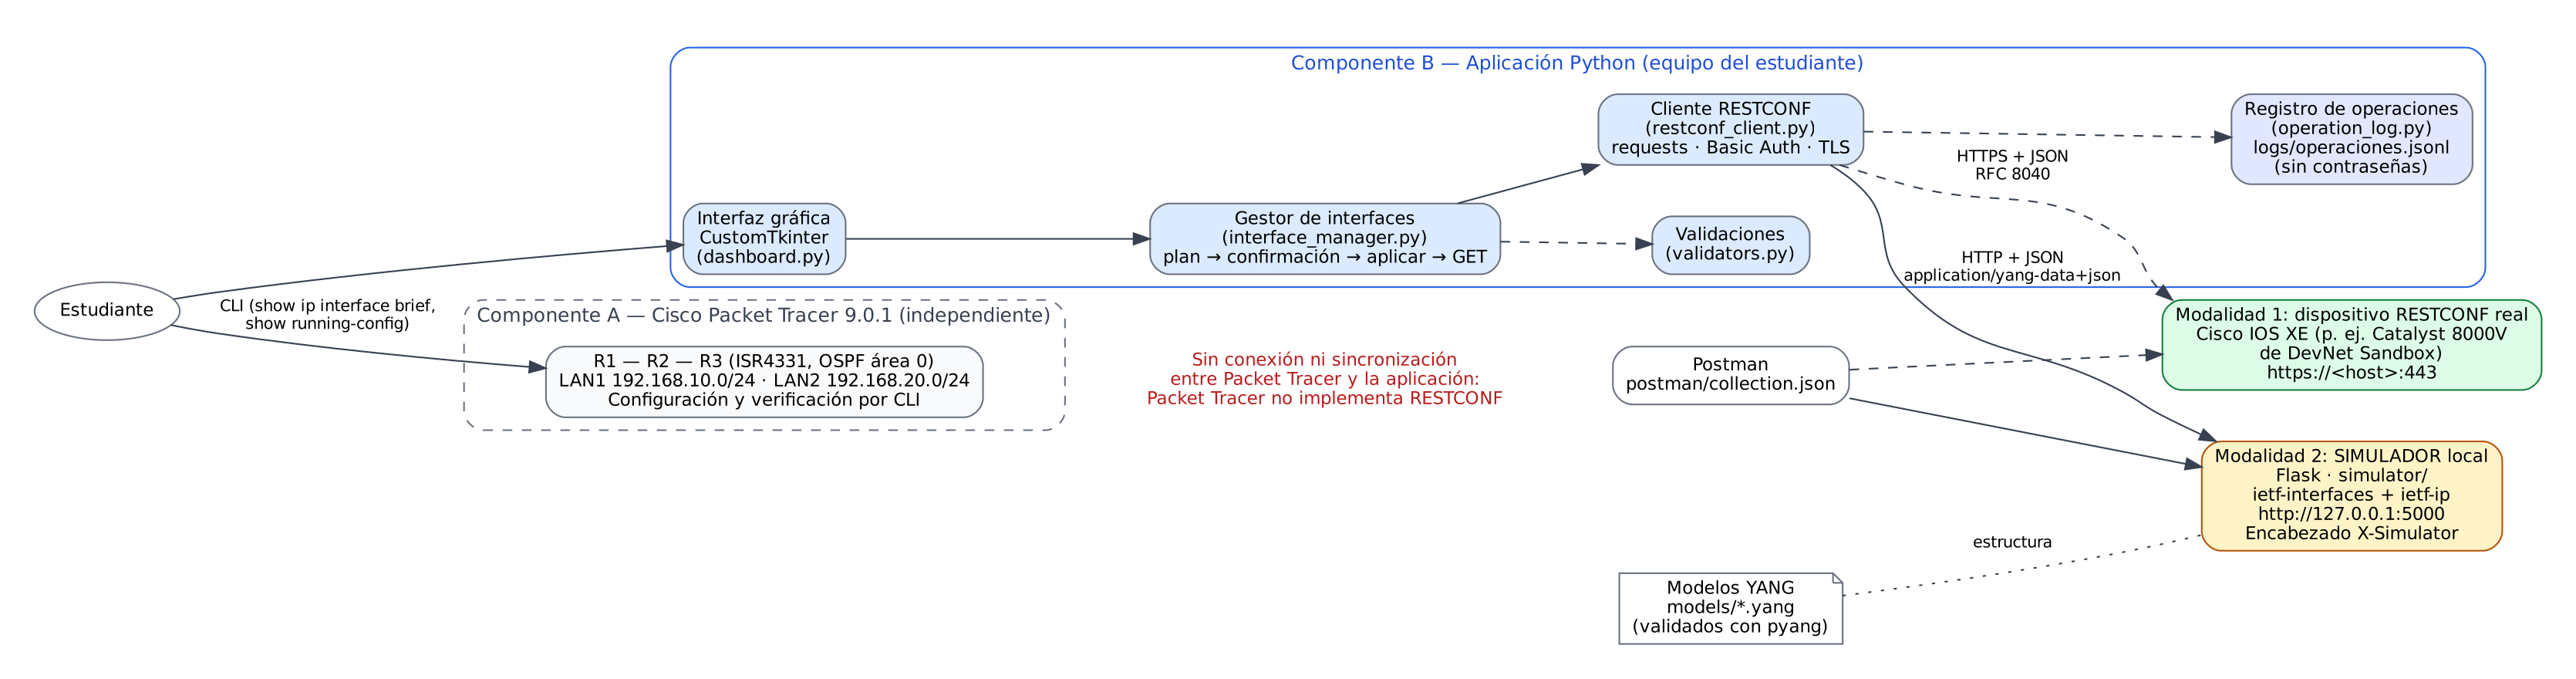
\includegraphics[width=\textwidth]{arquitectura.png}
  \caption{Arquitectura de la solución: aplicación Python, cliente RESTCONF, dispositivo real o simulador local, y laboratorio de Packet Tracer como entorno independiente.}
  \label{fig:arquitectura}
\end{figure}

\subsection{Herramientas y tecnologías}
\begin{table}[H]
\centering
\caption{Tecnologías utilizadas en el caso de uso}
\begin{tabularx}{\textwidth}{p{3.4cm}X}
\toprule
\textbf{Tecnología} & \textbf{Función dentro del proyecto} \\
\midrule
Cisco Packet Tracer 9.0.1 & Topología, configuración por CLI y verificación de conectividad \\
Python 3 & Lenguaje de la aplicación, del simulador y de las pruebas \\
Requests & Cliente HTTP para las solicitudes RESTCONF \\
Flask & Servidor del simulador RESTCONF \\
CustomTkinter & Interfaz gráfica de la aplicación \\
RESTCONF (RFC 8040) & Protocolo de administración programable \\
YANG: \texttt{ietf-interfaces}, \texttt{ietf-ip} & Modelos de los datos consultados y modificados \\
Pyang & Validación y exploración de los módulos YANG \\
Postman & Pruebas manuales de la API \\
pytest & Pruebas automatizadas \\
Git y GitHub & Control de versiones \parencite{repositorio} \\
\bottomrule
\end{tabularx}
\end{table}

\subsection{Topología del laboratorio}
La topología está formada por tres routers ISR4331 conectados en línea, dos switches 2960 y dos PC, uno en cada LAN (Figura~\ref{fig:topologia}). El enrutamiento es dinámico con OSPFv2 (proceso 1, área 0); las interfaces de LAN se declaran pasivas para no enviar mensajes OSPF hacia los usuarios. Se eligió el ISR4331 porque es el router de Packet Tracer que ejecuta IOS XE y porque sus nombres de interfaz coinciden con los del simulador. El archivo de la topología se encuentra en el repositorio como \texttt{lab/topologia\_ce5301.pkt}.

\begin{figure}[H]
  \centering
  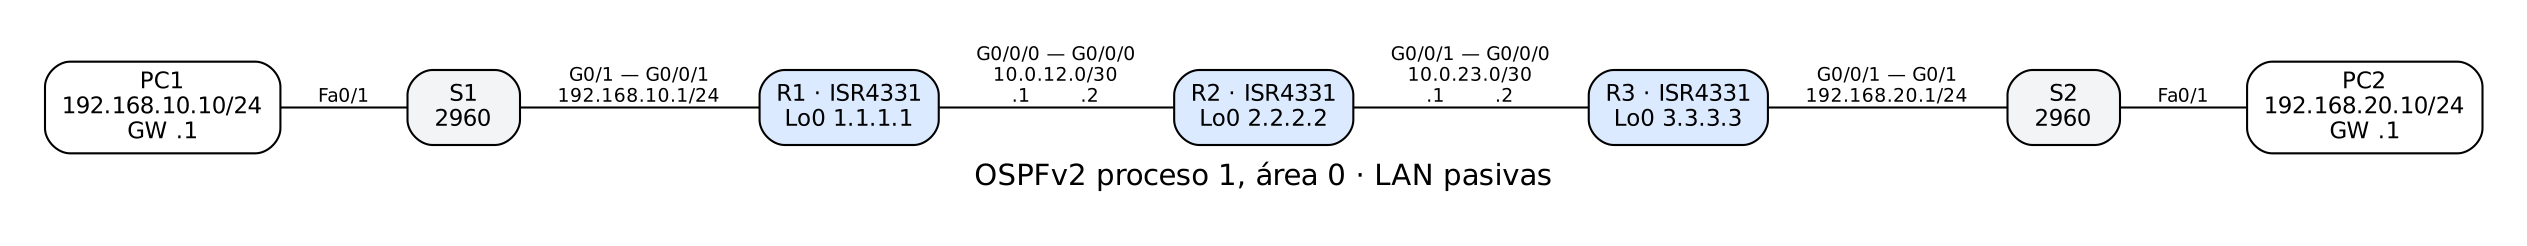
\includegraphics[width=\textwidth]{topologia.png}
  \caption{Topología implementada en Packet Tracer 9.0.1.}
  \label{fig:topologia}
\end{figure}

\subsection{Direccionamiento y dispositivos}
\begin{longtable}{p{1.5cm}p{2.0cm}p{2.6cm}p{3.2cm}p{3.9cm}}
\caption{Plan de direccionamiento del laboratorio}\\
\toprule
\textbf{Equipo} & \textbf{Interfaz} & \textbf{Dirección IP} & \textbf{Máscara} & \textbf{Función} \\
\midrule
\endfirsthead
\toprule
\textbf{Equipo} & \textbf{Interfaz} & \textbf{Dirección IP} & \textbf{Máscara} & \textbf{Función} \\
\midrule
\endhead
R1 & G0/0/0 & 10.0.12.1 & 255.255.255.252 & Enlace WAN hacia R2 \\
R1 & G0/0/1 & 192.168.10.1 & 255.255.255.0 & Puerta de enlace de LAN1 \\
R1 & Loopback0 & 1.1.1.1 & 255.255.255.255 & Router-ID OSPF \\
R2 & G0/0/0 & 10.0.12.2 & 255.255.255.252 & Enlace WAN hacia R1 \\
R2 & G0/0/1 & 10.0.23.1 & 255.255.255.252 & Enlace WAN hacia R3 \\
R2 & Loopback0 & 2.2.2.2 & 255.255.255.255 & Router-ID OSPF \\
R3 & G0/0/0 & 10.0.23.2 & 255.255.255.252 & Enlace WAN hacia R2 \\
R3 & G0/0/1 & 192.168.20.1 & 255.255.255.0 & Puerta de enlace de LAN2 \\
R3 & Loopback0 & 3.3.3.3 & 255.255.255.255 & Router-ID OSPF \\
R1--R3 & G0/0/2 & --- & --- & Sin uso (\texttt{shutdown}) \\
PC1 & Fa0 & 192.168.10.10 & 255.255.255.0 & Equipo final, gateway 192.168.10.1 \\
PC2 & Fa0 & 192.168.20.10 & 255.255.255.0 & Equipo final, gateway 192.168.20.1 \\
S1, S2 & --- & --- & --- & Switches de acceso (capa 2) \\
\bottomrule
\end{longtable}

\subsection{Flujo de funcionamiento}
\begin{enumerate}
  \item Configurar la topología y comprobar la conectividad en Packet Tracer.
  \item Iniciar la aplicación Python y seleccionar el modo de conexión (simulador o real).
  \item Autenticar contra el dispositivo o el simulador mediante \texttt{GET /restconf}.
  \item Consultar la configuración y el estado de las interfaces (recursos \texttt{interfaces} e \texttt{interfaces-state} del módulo \texttt{ietf-interfaces}).
  \item Presentar nombre, descripción, dirección IP, prefijo y estados administrativo y operativo.
  \item Seleccionar una interfaz y solicitar una modificación; la aplicación valida los datos.
  \item Mostrar la solicitud exacta (método, endpoint y JSON) y pedir confirmación.
  \item Enviar PATCH (descripción o habilitación) o PUT (dirección IP).
  \item Ejecutar un GET posterior y comparar el resultado con el cambio esperado.
  \item Registrar fecha, modo, operación, método, endpoint, código HTTP, resultado y tiempo de respuesta, sin almacenar credenciales.
\end{enumerate}

\subsection{Implementación}
La aplicación se organizó en módulos con responsabilidades separadas:
\begin{itemize}
  \item \texttt{restconf\_client.py}: construye las solicitudes con \texttt{requests}, maneja autenticación básica, TLS y tiempos de espera, y clasifica cada resultado como éxito, error HTTP, \textit{timeout}, falta de conectividad, error TLS o respuesta malformada. Nunca propaga excepciones de red a la interfaz gráfica.
  \item \texttt{interface\_manager.py}: combina configuración y estado, prepara cada cambio como un plan con el método, el endpoint y el cuerpo exactos, lo aplica y lo verifica con un GET.
  \item \texttt{validators.py}: valida direcciones IP, prefijos, descripciones (máximo 200 caracteres, como IOS) y datos de conexión antes de enviar cualquier solicitud.
  \item \texttt{operation\_log.py}: registra cada operación en formato JSON Lines y permite exportarla a CSV; no guarda contraseñas, encabezados de autorización ni cuerpos.
  \item \texttt{dashboard.py}: interfaz gráfica en CustomTkinter; ejecuta las operaciones de red en hilos secundarios para no bloquear la ventana.
\end{itemize}

\textbf{Decisión PATCH o PUT.} Para la descripción y la habilitación se usa PATCH, que combina el cuerpo con el recurso y modifica solo las hojas enviadas. Para la dirección IP se usa PUT: la lista \texttt{address} tiene como clave la propia IP, por lo que un \textit{merge} con una dirección distinta agregaría una entrada en lugar de reemplazarla. La aplicación lee la entrada completa, sustituye la dirección y reemplaza la entrada, conservando las demás hojas \parencite{rfc8040}.

\textbf{Configuración y estado.} Aunque el RFC 8343 integra el estado operativo en \texttt{/interfaces}, Cisco IOS XE expone la configuración en \texttt{ietf-interfaces:interfaces} y el estado en \texttt{interfaces-state}. La aplicación consulta ambos recursos y los combina; el simulador reproduce ese comportamiento. Si un dispositivo no ofrece el estado, la aplicación muestra los datos de configuración y lo indica.

\textbf{Simulador.} Implementado con Flask, expone el descubrimiento de la raíz RESTCONF, GET de interfaces y de estado, y PATCH y PUT sobre una interfaz. Valida los cuerpos contra la estructura de los modelos (hojas desconocidas o de solo lectura, tipos, clave que no coincide con la URI, IPv4 válida, máscara contigua, direcciones de red o broadcast y superposición de subredes) y responde con el formato de errores del RFC 8040. Cada respuesta incluye el encabezado \texttt{X-Simulator}. Los datos iniciales son ficticios y se inspiraron en el plan de direccionamiento de R1; no se sincronizan con Packet Tracer.

\begin{figure}[H]
  \centering
  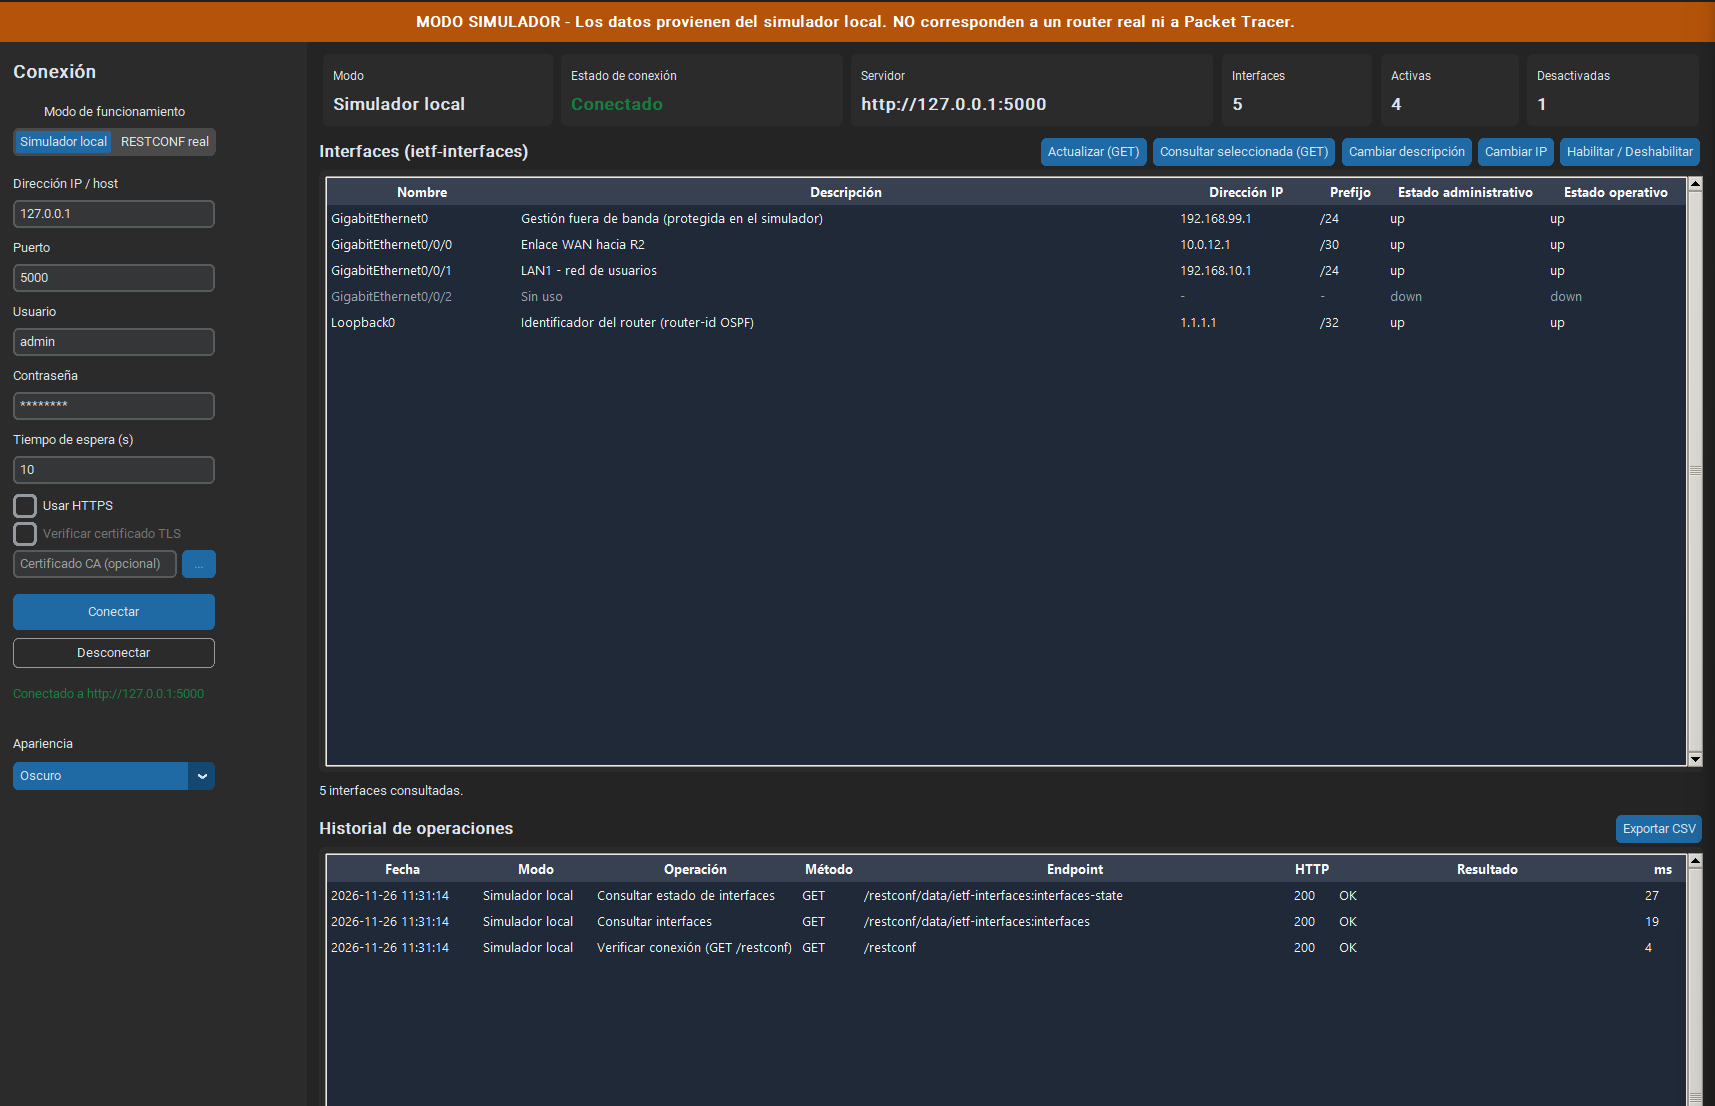
\includegraphics[width=0.95\textwidth]{01_panel_principal_modo_simulador.png}
  \caption{Panel principal de la aplicación en modo simulador. La franja superior indica que los datos no provienen de un router real.}
  \label{fig:gui1}
\end{figure}

\begin{figure}[H]
  \centering
  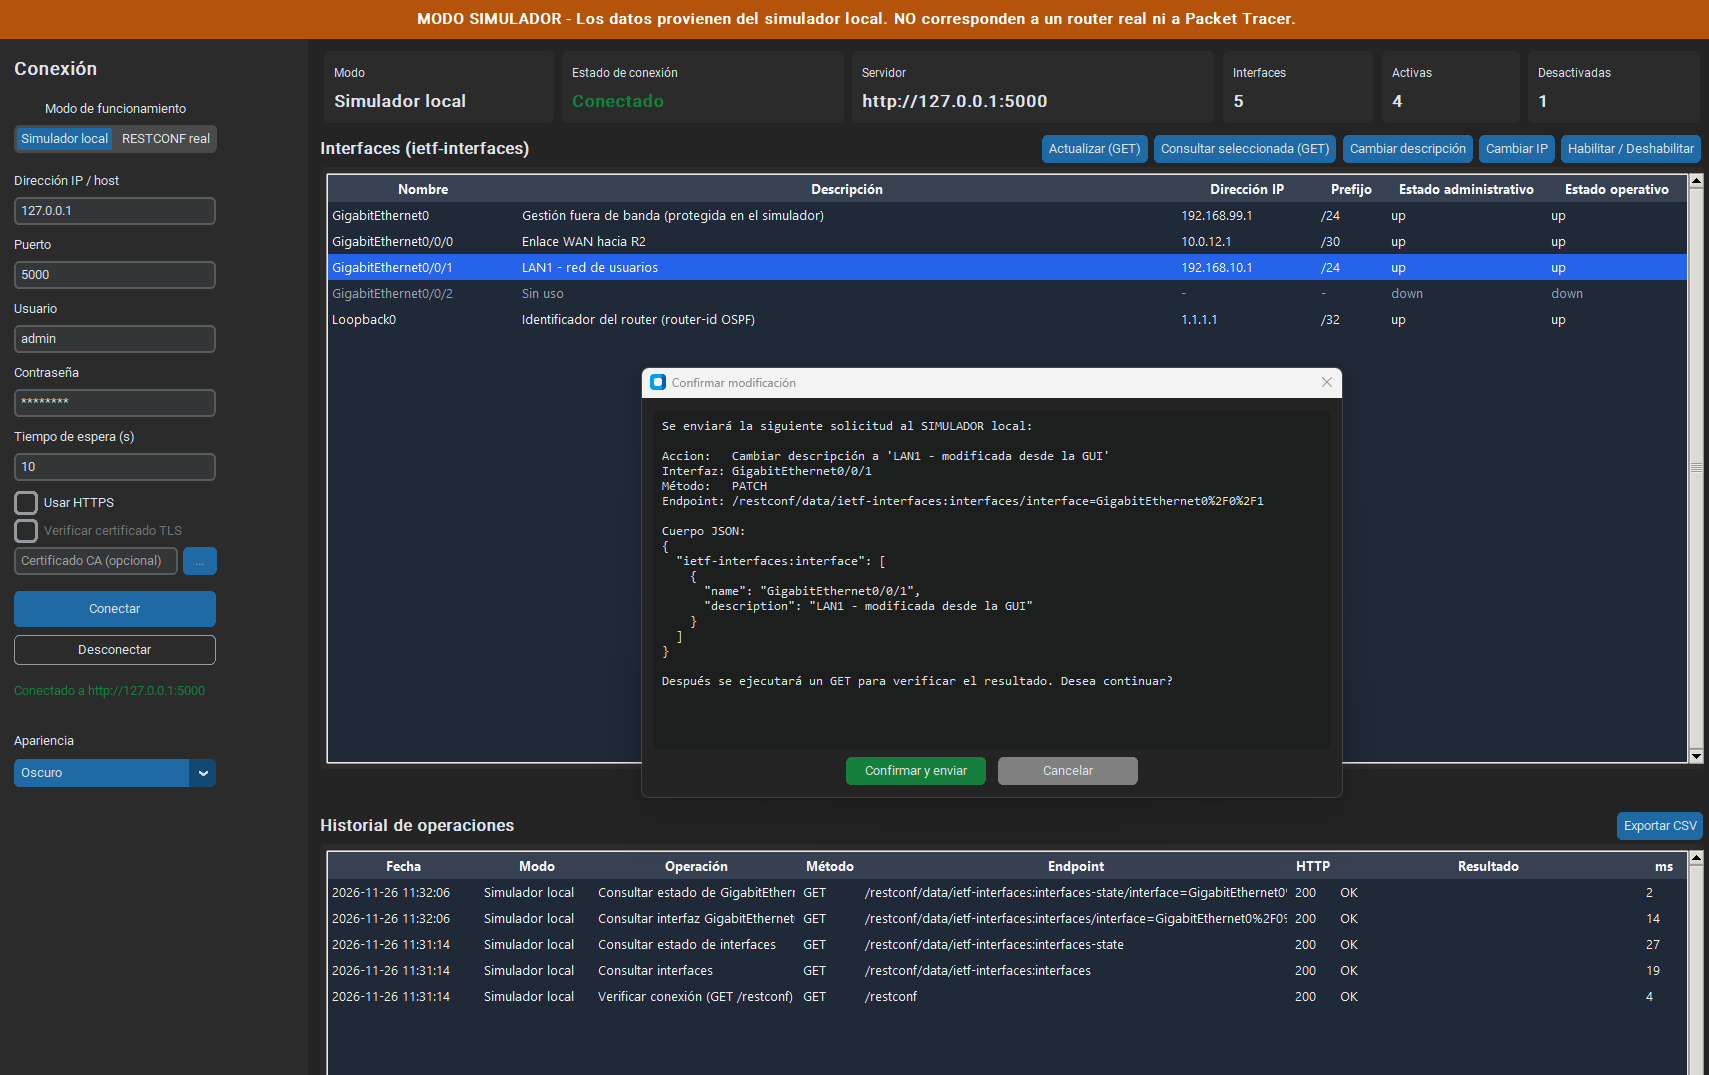
\includegraphics[width=0.95\textwidth]{02_confirmacion_antes_de_PATCH.png}
  \caption{Confirmación previa: la aplicación muestra el método, el endpoint y el cuerpo JSON exactos antes de enviar el PATCH.}
  \label{fig:gui2}
\end{figure}

\subsection{Pruebas diseñadas}
\begin{longtable}{p{0.8cm}p{3.6cm}p{4.4cm}p{4.6cm}}
\caption{Plan de pruebas del caso de uso y resultado obtenido}\label{tab:pruebas}\\
\toprule
\textbf{ID} & \textbf{Prueba} & \textbf{Procedimiento} & \textbf{Resultado obtenido} \\
\midrule
\endfirsthead
\toprule
\textbf{ID} & \textbf{Prueba} & \textbf{Procedimiento} & \textbf{Resultado obtenido} \\
\midrule
\endhead
P01 & Conectividad en Packet Tracer & \texttt{ping} y \texttt{tracert} de PC1 a PC2 & 3/4 respuestas (el primer eco se pierde por ARP); ruta R1--R2--R3 \\
P02 & Consulta de interfaces & GET al recurso \texttt{interfaces} del módulo \texttt{ietf-interfaces} & HTTP 200 con 5 interfaces (simulador) \\
P03 & Consulta individual & GET de \texttt{GigabitEthernet0/0/1} con la clave codificada & HTTP 200 con la interfaz solicitada (simulador) \\
P04 & Modificación de descripción & PATCH con una nueva descripción & HTTP 204 (simulador) \\
P05 & Verificación posterior & GET después del PATCH & La descripción coincide con el cambio (simulador) \\
P06 & Recurso inexistente & GET de \texttt{GigabitEthernet9/9/9} & HTTP 404 con mensaje controlado (simulador) \\
P07 & Credenciales incorrectas & Solicitud con contraseña errónea & HTTP 401; la contraseña no aparece en el registro (simulador) \\
P08 & Solicitud inválida & JSON mal formado e IP fuera del modelo & HTTP 400 en ambos casos; no se aplican cambios (simulador) \\
\bottomrule
\end{longtable}

Además del plan anterior, el conjunto de pruebas automatizadas (pytest) cubre los errores 403, 405, 415 y 500, el agotamiento del tiempo de espera, la falta de conectividad, las respuestas malformadas, el cambio de IP con PUT, la habilitación y deshabilitación de interfaces y el registro de operaciones.

\subsection{Video de demostración}
\textbf{Enlace:} \pendiente{insertar el enlace al video final.}

El video tendrá una duración máxima de diez minutos. Todas las personas integrantes participan y muestran su cámara durante su parte. El guion se resume en la Tabla~\ref{tab:guion}; la versión detallada está en \texttt{docs/guion\_demo.md} del repositorio.

\begin{longtable}{p{2.1cm}p{3.6cm}p{8.4cm}}
\caption{Guion del video de demostración}\label{tab:guion}\\
\toprule
\textbf{Tiempo} & \textbf{Integrante} & \textbf{Contenido} \\
\midrule
\endfirsthead
\toprule
\textbf{Tiempo} & \textbf{Integrante} & \textbf{Contenido} \\
\midrule
\endhead
0:00--1:30 & Giancarlo Vega & Presentación del equipo, problema y conceptos (YANG, RESTCONF, JSON) con el diagrama de arquitectura \\
1:30--3:30 & José Manuel Loría & Laboratorio en Packet Tracer: topología, OSPF, \texttt{show ip interface brief}, ping y \texttt{tracert}; rechazo de \texttt{restconf} en el ISR4331 \\
3:30--4:30 & Marco Villatoro & Modelos YANG con pyang y funcionamiento del simulador \\
4:30--7:00 & César Mora & Demostración de la aplicación: conexión, consulta, cambio de descripción con confirmación y verificación, deshabilitar una interfaz, historial \\
7:00--8:45 & Mariana Rojas & Manejo de errores (401, 403, IP inválida, sin conectividad), Postman y pruebas automatizadas \\
8:45--10:00 & Giancarlo Vega & Resultados, limitaciones, uso con un dispositivo real y conclusiones \\
\bottomrule
\end{longtable}

% ----------------------------------------------------------------------
% RESULTADOS
% ----------------------------------------------------------------------
\section{Resultados obtenidos y análisis de resultados}

\subsection{Resultados de conectividad y laboratorio}
Las configuraciones de los cinco equipos se aplicaron sin errores de sintaxis en Packet Tracer 9.0.1. Los Listados~\ref{lst:r1brief} a \ref{lst:ping} reproducen las salidas obtenidas el 25 de noviembre de 2026, transcritas de la CLI del simulador; las salidas completas se encuentran en \texttt{evidence/packet\_tracer/salidas\_cli.md}.

\begin{lstlisting}[language={},caption={R1: estado de interfaces},label={lst:r1brief}]
R1#show ip interface brief
Interface              IP-Address      OK? Method Status                Protocol
GigabitEthernet0/0/0   10.0.12.1       YES manual up                    up
GigabitEthernet0/0/1   192.168.10.1    YES manual up                    up
GigabitEthernet0/0/2   unassigned      YES unset  administratively down down
Loopback0              1.1.1.1         YES manual up                    up
\end{lstlisting}

\begin{figure}[H]
  \centering
  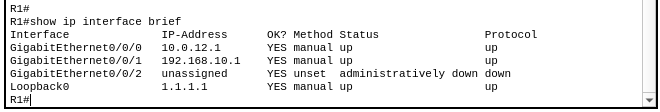
\includegraphics[width=\textwidth]{../../evidence/packet_tracer/show_ip_interface_brief_R1.png}
  \caption{Estado administrativo y operativo de las interfaces de R1 en Packet Tracer.}
  \label{fig:ip_int_R1}
\end{figure}

\begin{figure}[H]
  \centering
  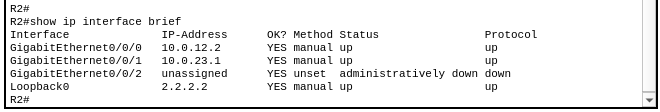
\includegraphics[width=\textwidth]{../../evidence/packet_tracer/show_ip_interface_brief_R2.png}
  \caption{Estado administrativo y operativo de las interfaces de R2 en Packet Tracer.}
  \label{fig:ip_int_R2}
\end{figure}

\begin{figure}[H]
  \centering
  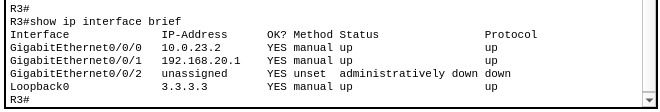
\includegraphics[width=\textwidth]{../../evidence/packet_tracer/show_ip_interface_brief_R3.png}
  \caption{Estado administrativo y operativo de las interfaces de R3 en Packet Tracer.}
  \label{fig:ip_int_R3}
\end{figure}

\begin{lstlisting}[language={},caption={R2: vecinos OSPF},label={lst:r2ospf}]
R2>show ip ospf neighbor

Neighbor ID     Pri   State           Dead Time   Address         Interface
3.3.3.3           1   FULL/DR         00:00:30    10.0.23.2       GigabitEthernet0/0/1
1.1.1.1           1   FULL/BDR        00:00:33    10.0.12.1       GigabitEthernet0/0/0
\end{lstlisting}

\begin{figure}[H]
  \centering
  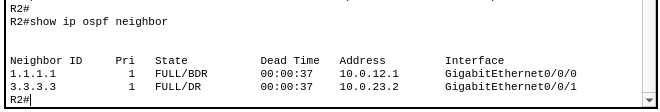
\includegraphics[width=\textwidth]{../../evidence/packet_tracer/show_ip_ospf_neighfor_R2.png}
  \caption{Verificación de adyacencias OSPF en estado FULL.}
  \label{fig:ip_ospf_R2}
\end{figure}

\begin{lstlisting}[language={},caption={R1: rutas aprendidas por OSPF},label={lst:r1route}]
R1#show ip route ospf
     2.0.0.0/32 is subnetted, 1 subnets
O       2.2.2.2 [110/2] via 10.0.12.2, 00:05:24, GigabitEthernet0/0/0
     3.0.0.0/32 is subnetted, 1 subnets
O       3.3.3.3 [110/3] via 10.0.12.2, 00:04:37, GigabitEthernet0/0/0
     10.0.0.0/8 is variably subnetted, 3 subnets, 2 masks
O       10.0.23.0 [110/2] via 10.0.12.2, 00:04:47, GigabitEthernet0/0/0
O    192.168.20.0 [110/3] via 10.0.12.2, 00:04:37, GigabitEthernet0/0/0
\end{lstlisting}

\begin{figure}[H]
  \centering
  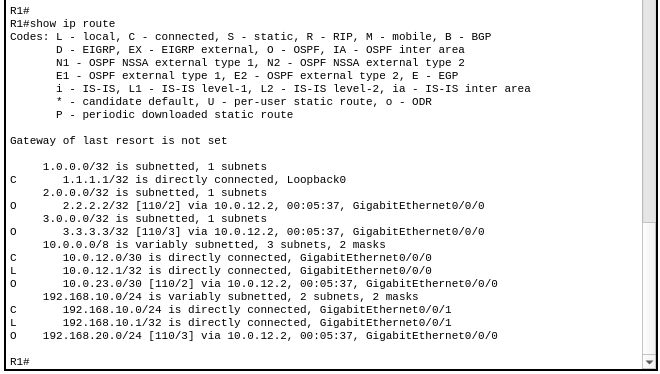
\includegraphics[width=\textwidth]{../../evidence/packet_tracer/show_ip_route_R1.png}
  \caption{Tabla de enrutamiento con rutas aprendidas vía OSPF entre redes remotas.}
  \label{fig:ip_route_R1}
\end{figure}

\begin{lstlisting}[language={},caption={PC1: conectividad extremo a extremo hacia PC2},label={lst:ping}]
C:\>ping 192.168.20.10
Request timed out.
Reply from 192.168.20.10: bytes=32 time<1ms TTL=125
Reply from 192.168.20.10: bytes=32 time<1ms TTL=125
Reply from 192.168.20.10: bytes=32 time<1ms TTL=125
    Packets: Sent = 4, Received = 3, Lost = 1 (25% loss),

C:\>tracert 192.168.20.10
  1   0 ms      0 ms      0 ms      192.168.10.1
  2   0 ms      0 ms      0 ms      10.0.12.2
  3   0 ms      0 ms      0 ms      10.0.23.2
  4   0 ms      0 ms      0 ms      192.168.20.10
\end{lstlisting}

\begin{figure}[H]
  \centering
  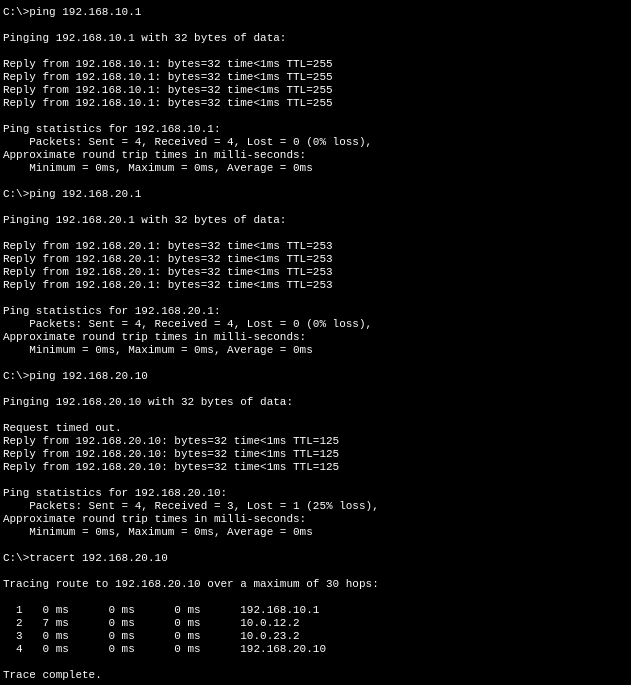
\includegraphics[width=\textwidth]{../../evidence/packet_tracer/ping_y_tracert_PC1.png}
  \caption{Prueba de conectividad y trazado de ruta en la topología.}
  \label{fig:ping_y_tracert_PC1}
\end{figure}

R2 mantiene adyacencias en estado \texttt{FULL} con R1 y R3, y R1 aprende por OSPF todas las redes remotas, incluida la LAN2, con costos coherentes con el número de saltos (110/2 hacia R2 y 110/3 hacia R3 y LAN2). El primer eco del ping se pierde mientras se resuelve ARP, comportamiento esperado. El valor \texttt{TTL=125} (128 menos 3) y la salida de \texttt{tracert} confirman que el tráfico atraviesa los tres routers. Las interfaces G0/0/2 aparecen \texttt{administratively down}, como se configuró.

\subsection{Resultados de las solicitudes API}
\textbf{Todos los resultados de esta sección se obtuvieron contra el simulador RESTCONF local, no contra un router real ni contra Packet Tracer.} Se generaron con el script \texttt{scripts/generar\_evidencias.py}, que guarda cada solicitud y respuesta HTTP exactas en \texttt{evidence/simulador/}.

\begin{longtable}{p{0.5cm}p{6.4cm}p{1.8cm}p{1.5cm}p{2.4cm}}
\caption{Solicitudes ejecutadas contra el simulador}\label{tab:api}\\
\toprule
\textbf{\#} & \textbf{Escenario} & \textbf{Método} & \textbf{HTTP} & \textbf{Tiempo (ms)} \\
\midrule
\endfirsthead
\toprule
\textbf{\#} & \textbf{Escenario} & \textbf{Método} & \textbf{HTTP} & \textbf{Tiempo (ms)} \\
\midrule
\endhead
1 & Consulta de todas las interfaces & GET & 200 & 7,56 \\
2 & Consulta de una interfaz & GET & 200 & 2,72 \\
3 & Estado operativo (\texttt{interfaces-state}) & GET & 200 & 2,19 \\
4 & Modificación de la descripción & PATCH & 204 & 2,43 \\
5 & Verificación posterior & GET & 200 & 2,58 \\
6 & Interfaz inexistente & GET & 404 & 1,71 \\
7 & Credenciales incorrectas & GET & 401 & 1,84 \\
8 & JSON mal formado & PATCH & 400 & 1,65 \\
9 & IP fuera del modelo (300.1.1.1) & PATCH & 400 & 1,90 \\
10 & Interfaz protegida & PATCH & 403 & 1,80 \\
11 & Método no permitido & DELETE & 405 & 1,88 \\
12 & Error interno inyectado & GET & 500 & 2,05 \\
13 & Cambio de IP con la entrada completa & PUT & 204 & 1,97 \\
\bottomrule
\end{longtable}

Cada tiempo corresponde a una única ejecución; el valor más alto (7,56~ms) es la primera solicitud tras iniciar el servidor, que incluye la preparación de la conexión. Las mediciones repetidas se analizan en la Sección~\ref{sec:cuantitativo}. El Listado~\ref{lst:patch} muestra el intercambio completo de los escenarios 4 y 5.

\begin{lstlisting}[language={},caption={PATCH de la descripción y GET de verificación (simulador)},label={lst:patch}]
PATCH /restconf/data/ietf-interfaces:interfaces/interface=GigabitEthernet0%2F0%2F1
Content-Type: application/yang-data+json
{"ietf-interfaces:interface": [{"name": "GigabitEthernet0/0/1",
  "description": "LAN1 - descripción modificada vía RESTCONF"}]}
-> HTTP 204 No Content

GET /restconf/data/ietf-interfaces:interfaces/interface=GigabitEthernet0%2F0%2F1
-> HTTP 200
{"ietf-interfaces:interface": [{
   "name": "GigabitEthernet0/0/1",
   "description": "LAN1 - descripción modificada vía RESTCONF",
   "type": "iana-if-type:ethernetCsmacd",
   "enabled": true,
   "ietf-ip:ipv4": {"address": [{"ip": "192.168.10.1", "netmask": "255.255.255.0"}]}}]}
\end{lstlisting}

Los errores se devuelven con la estructura del RFC 8040. Por ejemplo, la consulta de una interfaz inexistente produjo \texttt{error-type: application}, \texttt{error-tag: invalid-value} y un mensaje legible, que la aplicación muestra al usuario. La solicitud con una IP inválida fue rechazada con HTTP 400; una de las pruebas automatizadas confirma, con un GET posterior, que un cuerpo rechazado no modifica la configuración.

\begin{figure}[H]
  \centering
  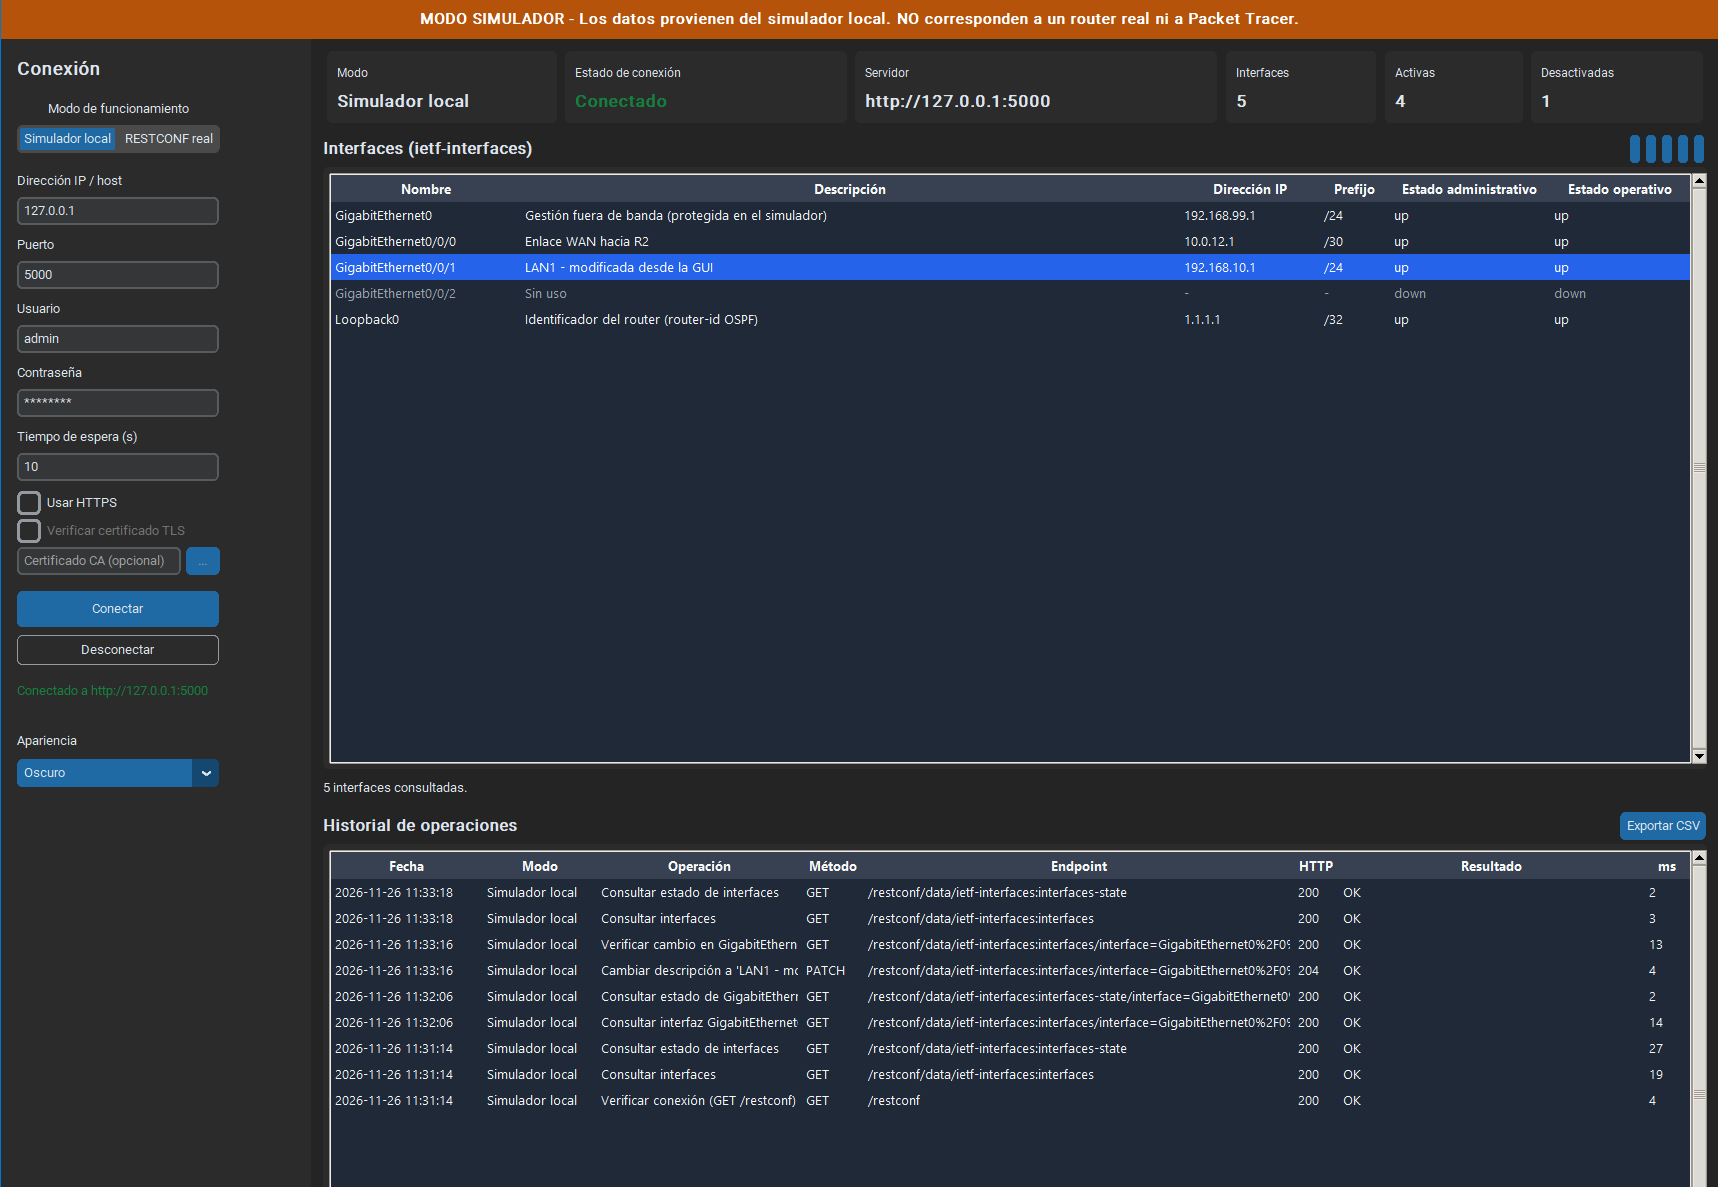
\includegraphics[width=0.95\textwidth]{03_resultado_verificado_e_historial.png}
  \caption{Resultado tras el cambio: la tabla refleja la nueva descripción y el historial registra el PATCH (HTTP 204) y el GET de verificación (HTTP 200). Datos del simulador.}
  \label{fig:gui3}
\end{figure}

\begin{figure}[H]
  \centering
  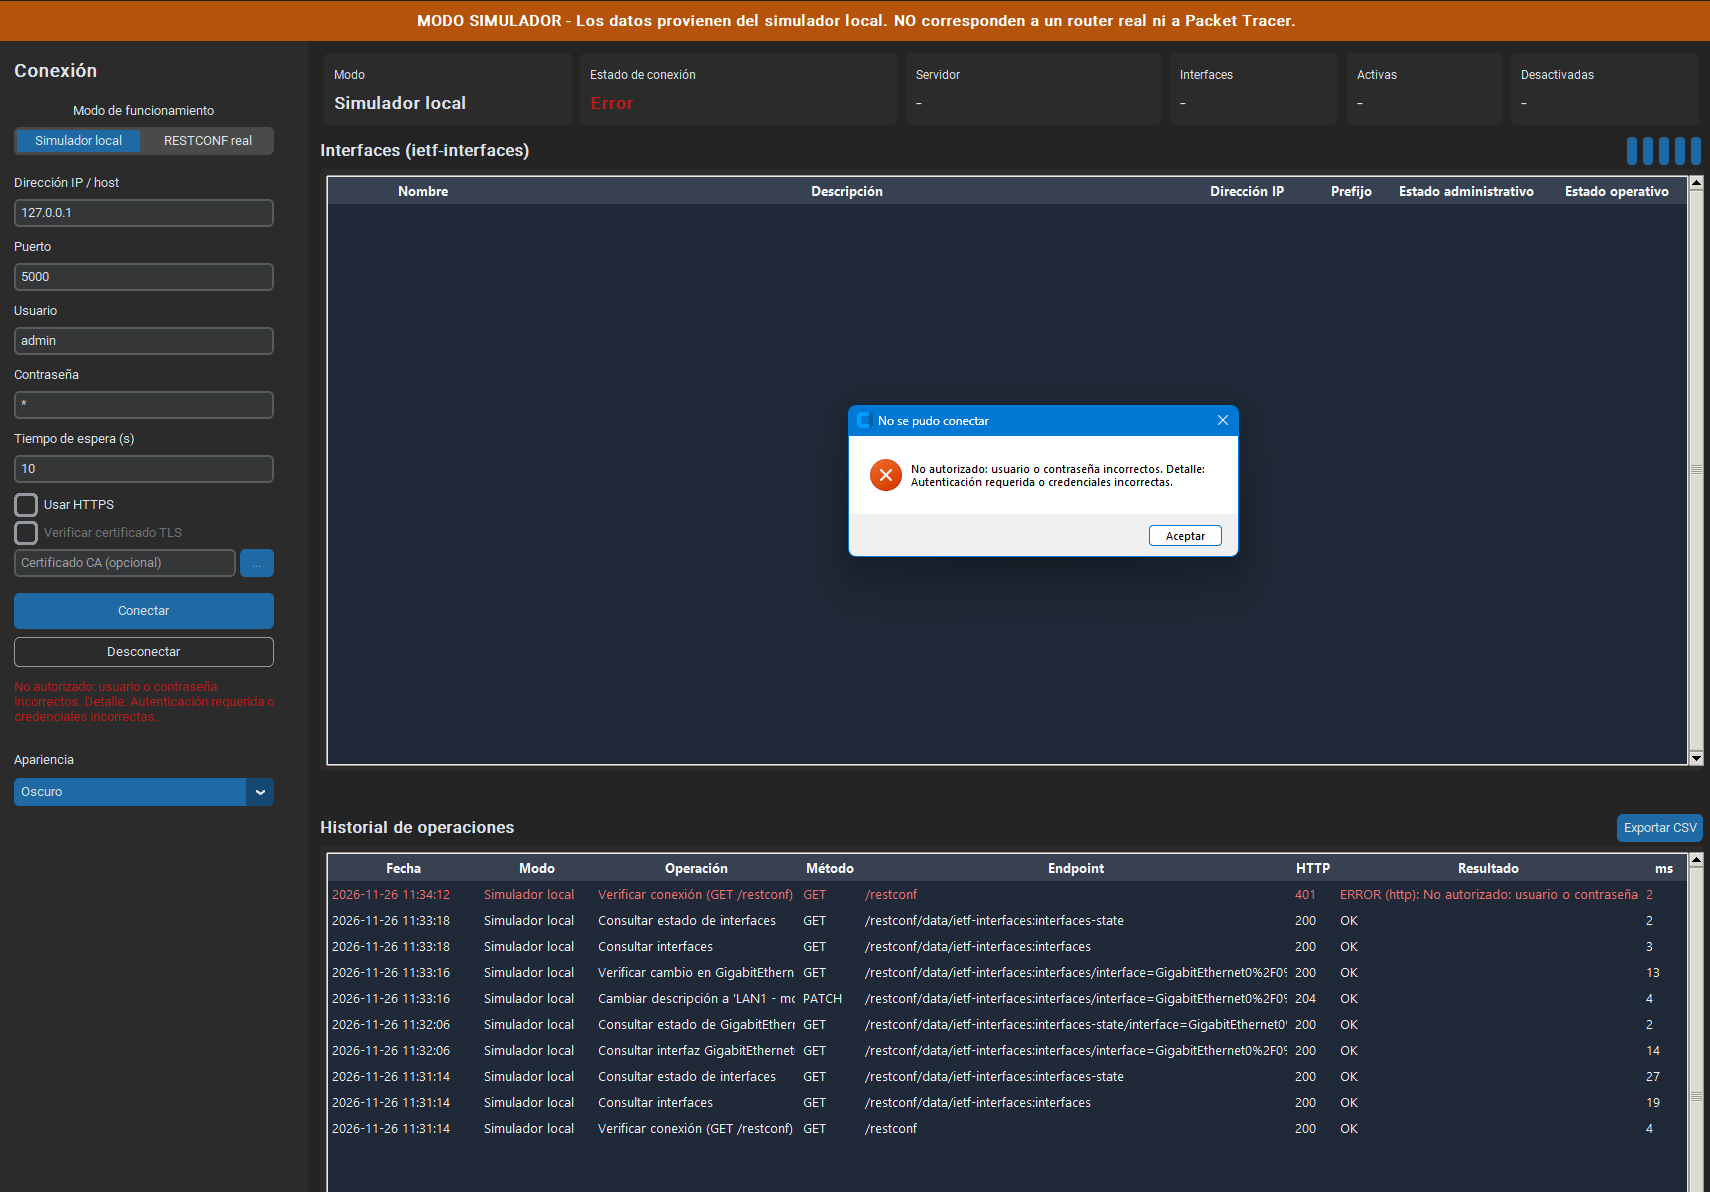
\includegraphics[width=0.95\textwidth]{04_error_401.png}
  \caption{Manejo de credenciales incorrectas: el simulador responde HTTP 401 y la aplicación muestra un mensaje controlado sin registrar la contraseña.}
  \label{fig:gui4}
\end{figure}

\textbf{Pruebas automatizadas.} La ejecución de \texttt{python -m pytest -v} terminó con \textbf{39 pruebas aprobadas y 5 omitidas}. Las omitidas son las pruebas contra un dispositivo real, que se ejecutan solo si se configura la variable \texttt{RESTCONF\_HOST}. La misma suite se ejecutó con Python 3.12 y con Python 3.10 con el mismo resultado. La colección de Postman se comprobó reproduciendo sus siete solicitudes contra el simulador; todas devolvieron el código esperado.

\subsection{Resultados contra un dispositivo IOS XE real}\label{sec:real}

\textbf{Entorno.} Para validar el modo \textit{RESTCONF real} se reservó el sandbox \textit{IOS XE on Catalyst 8000v} de Cisco DevNet, que ofrece un router virtual Catalyst 8000v con IOS XE 17.12.02 y NETCONF y RESTCONF habilitados. Es un entorno privado bajo reserva, con una duración máxima de dos días. Sus equipos usan direcciones privadas, por lo que solo son alcanzables mediante VPN \parencite{devnet_faq}. Se utilizó el cliente OpenConnect, alternativa de código abierto a Cisco Secure Client, cuya descarga requiere un contrato de soporte \parencite{devnet_faq}. Las pruebas se realizaron el 25 de noviembre de 2026.

Durante la conexión, OpenConnect autenticó correctamente pero no logró crear el adaptador de red virtual en Windows (\texttt{Set up tun device failed}), porque el nombre de interfaz que genera a partir del servidor era demasiado largo. Se resolvió asignando un nombre corto de interfaz en el perfil. Con la VPN activa, se comprobó con \texttt{Test-NetConnection} que el router (10.10.20.48) aceptaba conexiones en los puertos TCP 443 (RESTCONF) y 830 (NETCONF).

\textbf{Primera consulta.} Un GET a \texttt{/restconf/data/ietf-interfaces:interfaces} con \texttt{curl} devolvió HTTP 200 con siete interfaces. La respuesta no incluyó el encabezado \texttt{X-Simulator} y el servidor se identificó como \texttt{openresty}, lo que confirma que respondió el dispositivo real y no el simulador. El JSON tuvo la misma estructura que en el simulador, definida por \texttt{ietf-interfaces} e \texttt{ietf-ip}. También se observaron diferencias que el modelo admite: \texttt{Loopback0} no incluye la hoja opcional \texttt{description}, el tipo de las interfaces lógicas es \texttt{softwareLoopback} y el contenedor de presencia \texttt{ietf-ip:ipv6} aparece vacío.

\textbf{Pruebas automatizadas.} Las cinco pruebas de \texttt{tests/test\_real\_device.py} terminaron aprobadas en 5,38~s: descubrimiento, consulta de todas las interfaces, consulta individual, interfaz inexistente y PATCH de la descripción con restauración, esta última sobre \texttt{Loopback109}. Con ello, el conjunto completo suma 44 de 44 pruebas aprobadas: 39 contra el simulador y 5 contra el router real. Se registraron cuatro advertencias \texttt{InsecureRequestWarning}, esperables porque se desactivó la verificación del certificado autofirmado del sandbox.

\textbf{Operación con la aplicación.} Se ejecutó \texttt{python main.py --modo real} sin modificar el código. La franja superior cambia a azul e identifica el dispositivo real (Figura~\ref{fig:real_panel}). La Tabla~\ref{tab:api_real} resume las solicitudes registradas en el historial de la aplicación.

\begin{figure}[H]
  \centering
  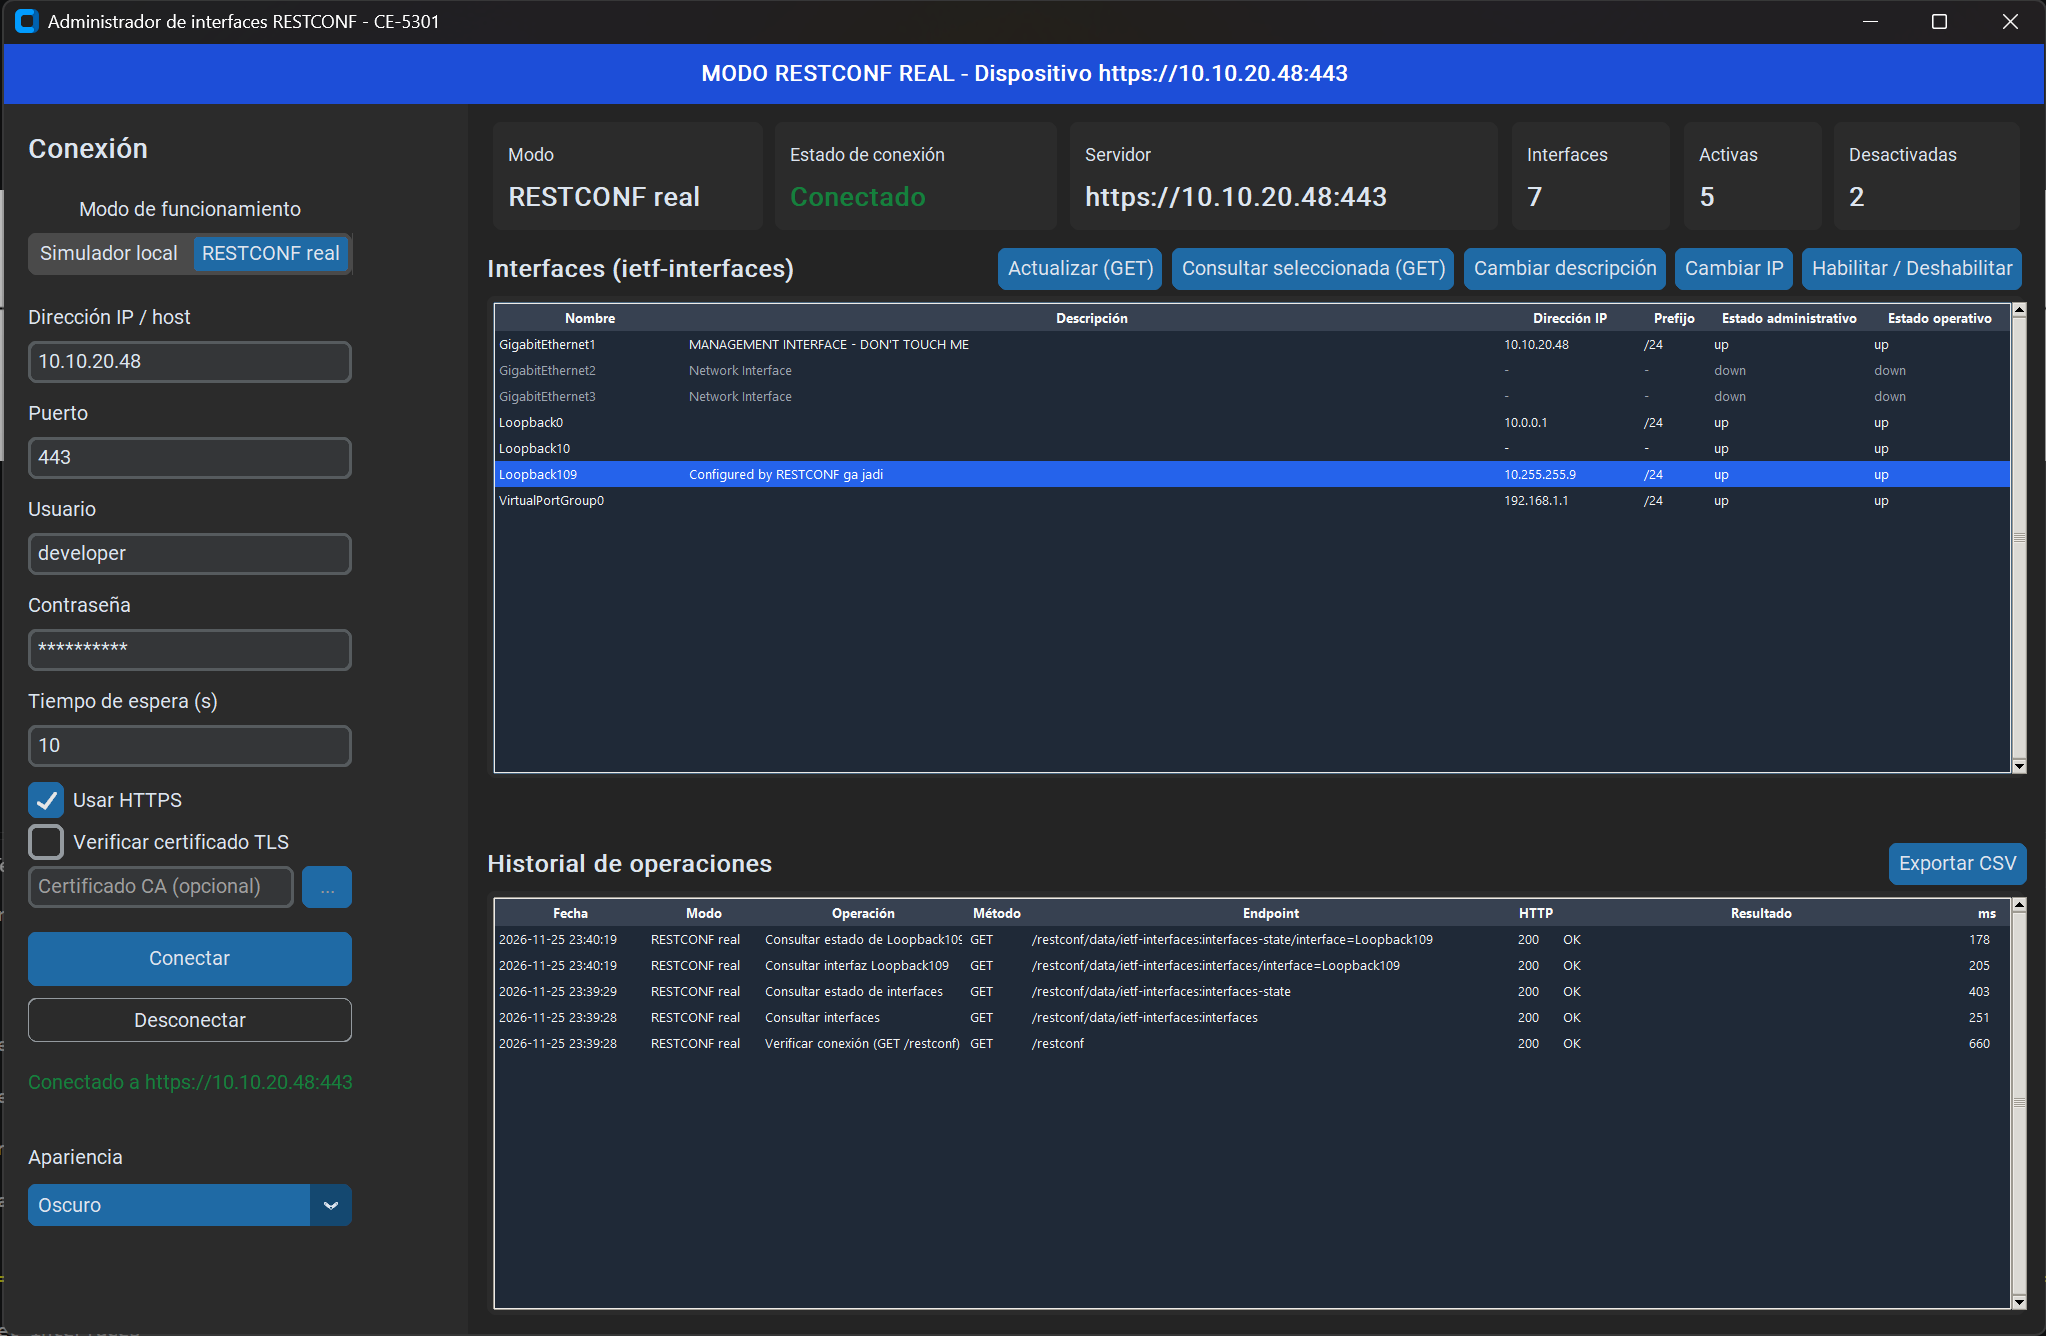
\includegraphics[width=0.95\textwidth]{cisco_simulador}
  \caption{Aplicación conectada en modo RESTCONF real al Catalyst 8000v de DevNet Sandbox.}
  \label{fig:real_panel}
\end{figure}

\begin{longtable}{p{0.5cm}p{6.6cm}p{1.6cm}p{1.3cm}p{2.4cm}}
\caption{Solicitudes ejecutadas contra el router real (historial de la aplicación)}\label{tab:api_real}\\
\toprule
\textbf{\#} & \textbf{Operación} & \textbf{Método} & \textbf{HTTP} & \textbf{Tiempo (ms)} \\
\midrule
\endfirsthead
\toprule
\textbf{\#} & \textbf{Operación} & \textbf{Método} & \textbf{HTTP} & \textbf{Tiempo (ms)} \\
\midrule
\endhead
1 & Verificación de conexión (\texttt{/restconf}) & GET & 200 & 660 \\
2 & Consulta de interfaces & GET & 200 & 251 \\
3 & Estado operativo (\texttt{interfaces-state}) & GET & 200 & 403 \\
4 & Consulta de \texttt{Loopback109} & GET & 200 & 205 \\
5 & Estado de \texttt{Loopback109} & GET & 200 & 178 \\
6 & Cambio de descripción de \texttt{Loopback109} & PATCH & 204 & 942 \\
7 & Verificación posterior & GET & 200 & 162 \\
8 & Restauración de la descripción original & PATCH & 204 & 580 \\
9 & Verificación posterior & GET & 200 & 162 \\
10 & Habilitación de \texttt{GigabitEthernet2} & PATCH & 204 & 638 \\
11 & Verificación posterior & GET & 200 & 176 \\
\bottomrule
\end{longtable}

Las once solicitudes terminaron con el código esperado. Antes de cada cambio, la aplicación mostró el método, el endpoint y el cuerpo JSON exactos (Figuras~\ref{fig:real_conf_marco} y \ref{fig:real_conf_default}). El cuerpo enviado al router es idéntico en estructura al usado con el simulador.

\begin{figure}[H]
  \centering
  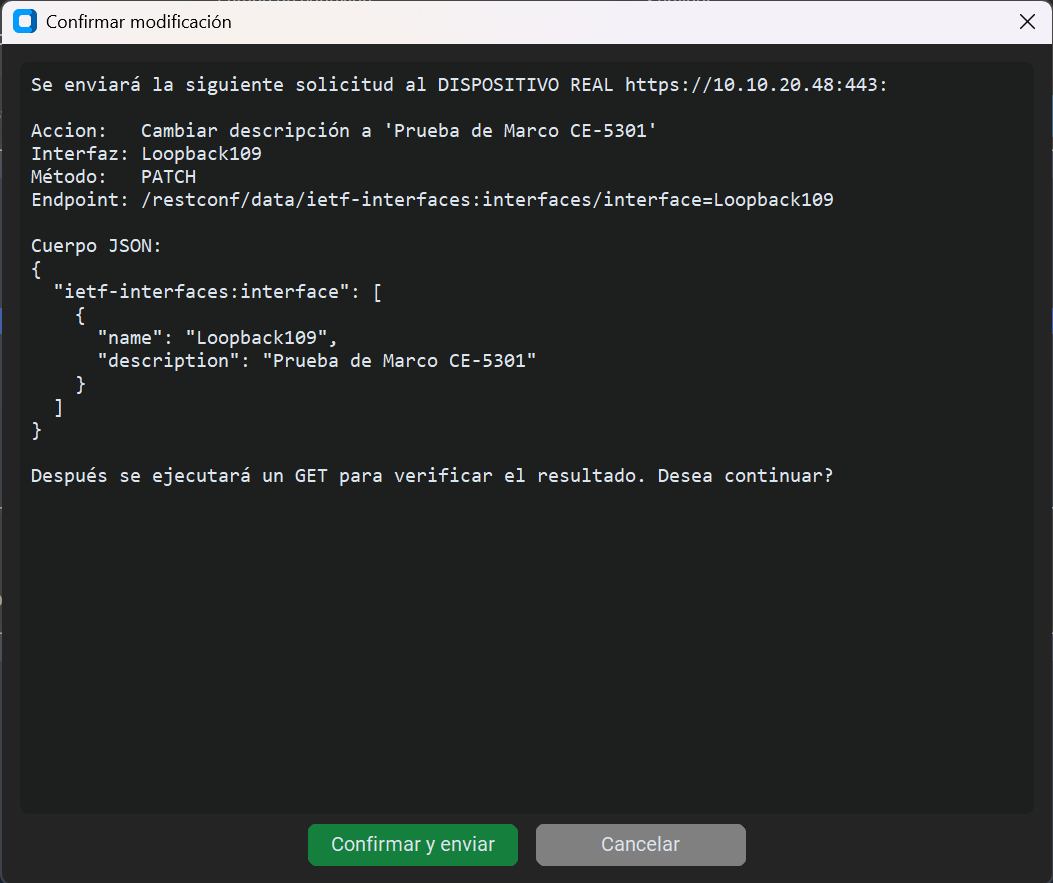
\includegraphics[width=0.7\textwidth]{cisco_loopback109_Marco}
  \caption{Confirmación previa al PATCH que cambia la descripción de Loopback109 en el router real.}
  \label{fig:real_conf_marco}
\end{figure}

\begin{figure}[H]
  \centering
  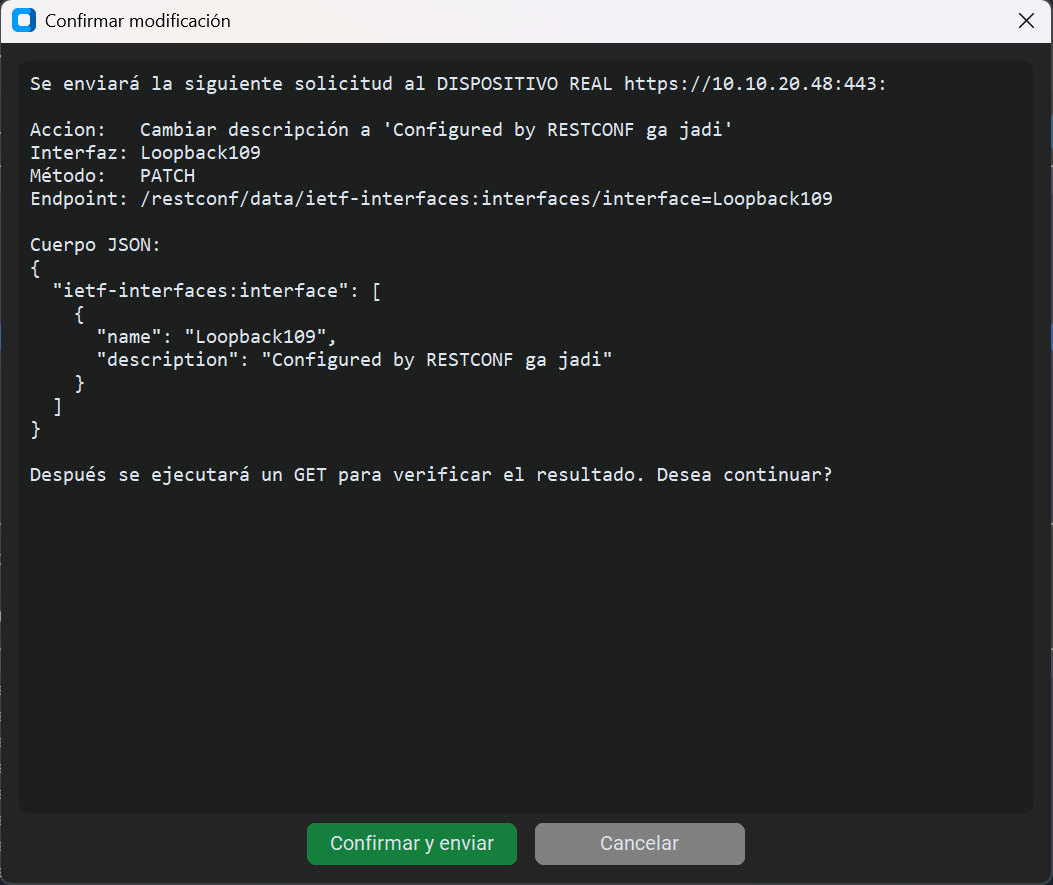
\includegraphics[width=0.7\textwidth]{cisco_loopback109_Default}
  \caption{Confirmación previa al PATCH que restaura la descripción original de Loopback109.}
  \label{fig:real_conf_default}
\end{figure}

\textbf{Estado administrativo frente a estado operativo.} Al habilitar \texttt{GigabitEthernet2} (Figura~\ref{fig:real_conf_gi2}), su estado administrativo pasó a \texttt{up}, pero el estado operativo reportado por el router fue \texttt{lower-layer-down} (Figura~\ref{fig:real_gi2}). La hoja \texttt{enabled} (\texttt{rw}) expresa la intención configurada, mientras que \texttt{oper-status} (\texttt{ro}) refleja la condición real de la interfaz. En este caso, la capa inferior no tiene enlace porque nada está conectado a esa interfaz virtual. \texttt{lower-layer-down} es uno de los valores definidos en la enumeración \texttt{oper-status} de \texttt{ietf-interfaces} \parencite{rfc8343}. Este comportamiento no puede observarse en el simulador, que deriva el estado operativo directamente de la configuración. Al finalizar, la interfaz se deshabilitó nuevamente para dejar el equipo en su estado original.

\begin{figure}[H]
  \centering
  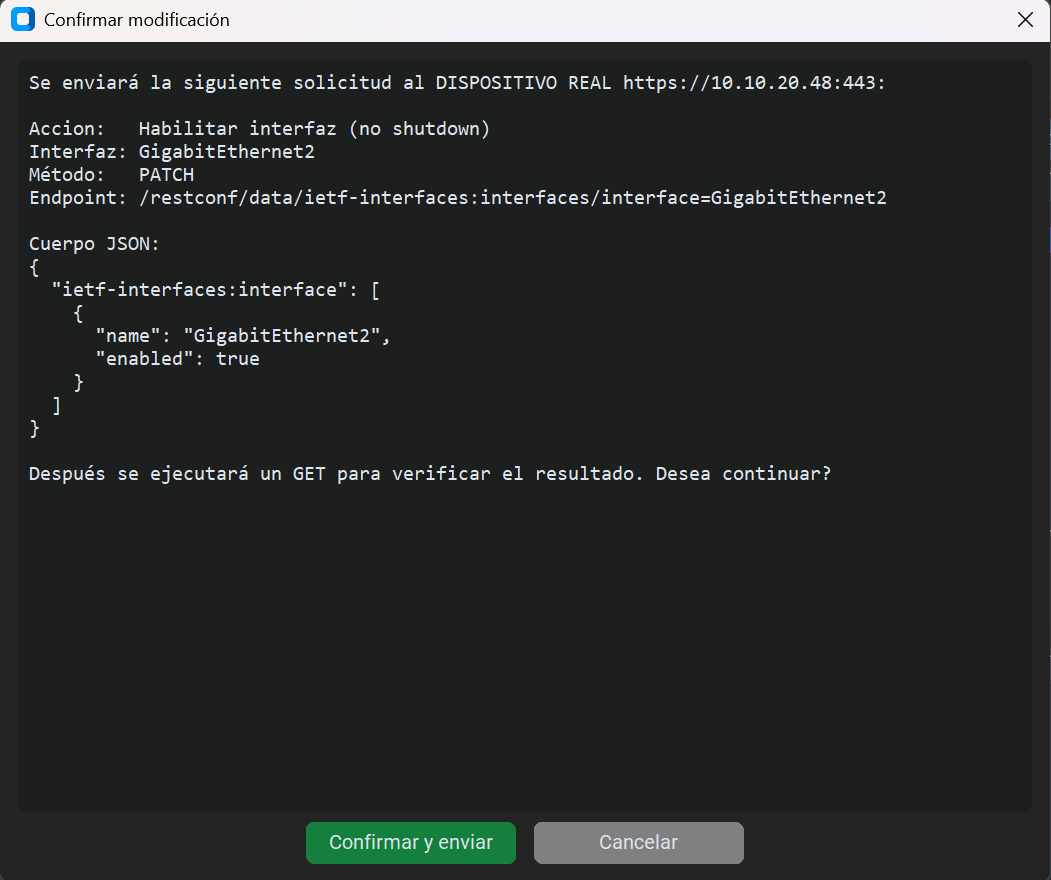
\includegraphics[width=0.7\textwidth]{cisco_GB_habilitar_deshabilitar}
  \caption{Confirmación previa al PATCH que habilita GigabitEthernet2 (\texttt{"enabled": true}).}
  \label{fig:real_conf_gi2}
\end{figure}

\begin{figure}[H]
  \centering
  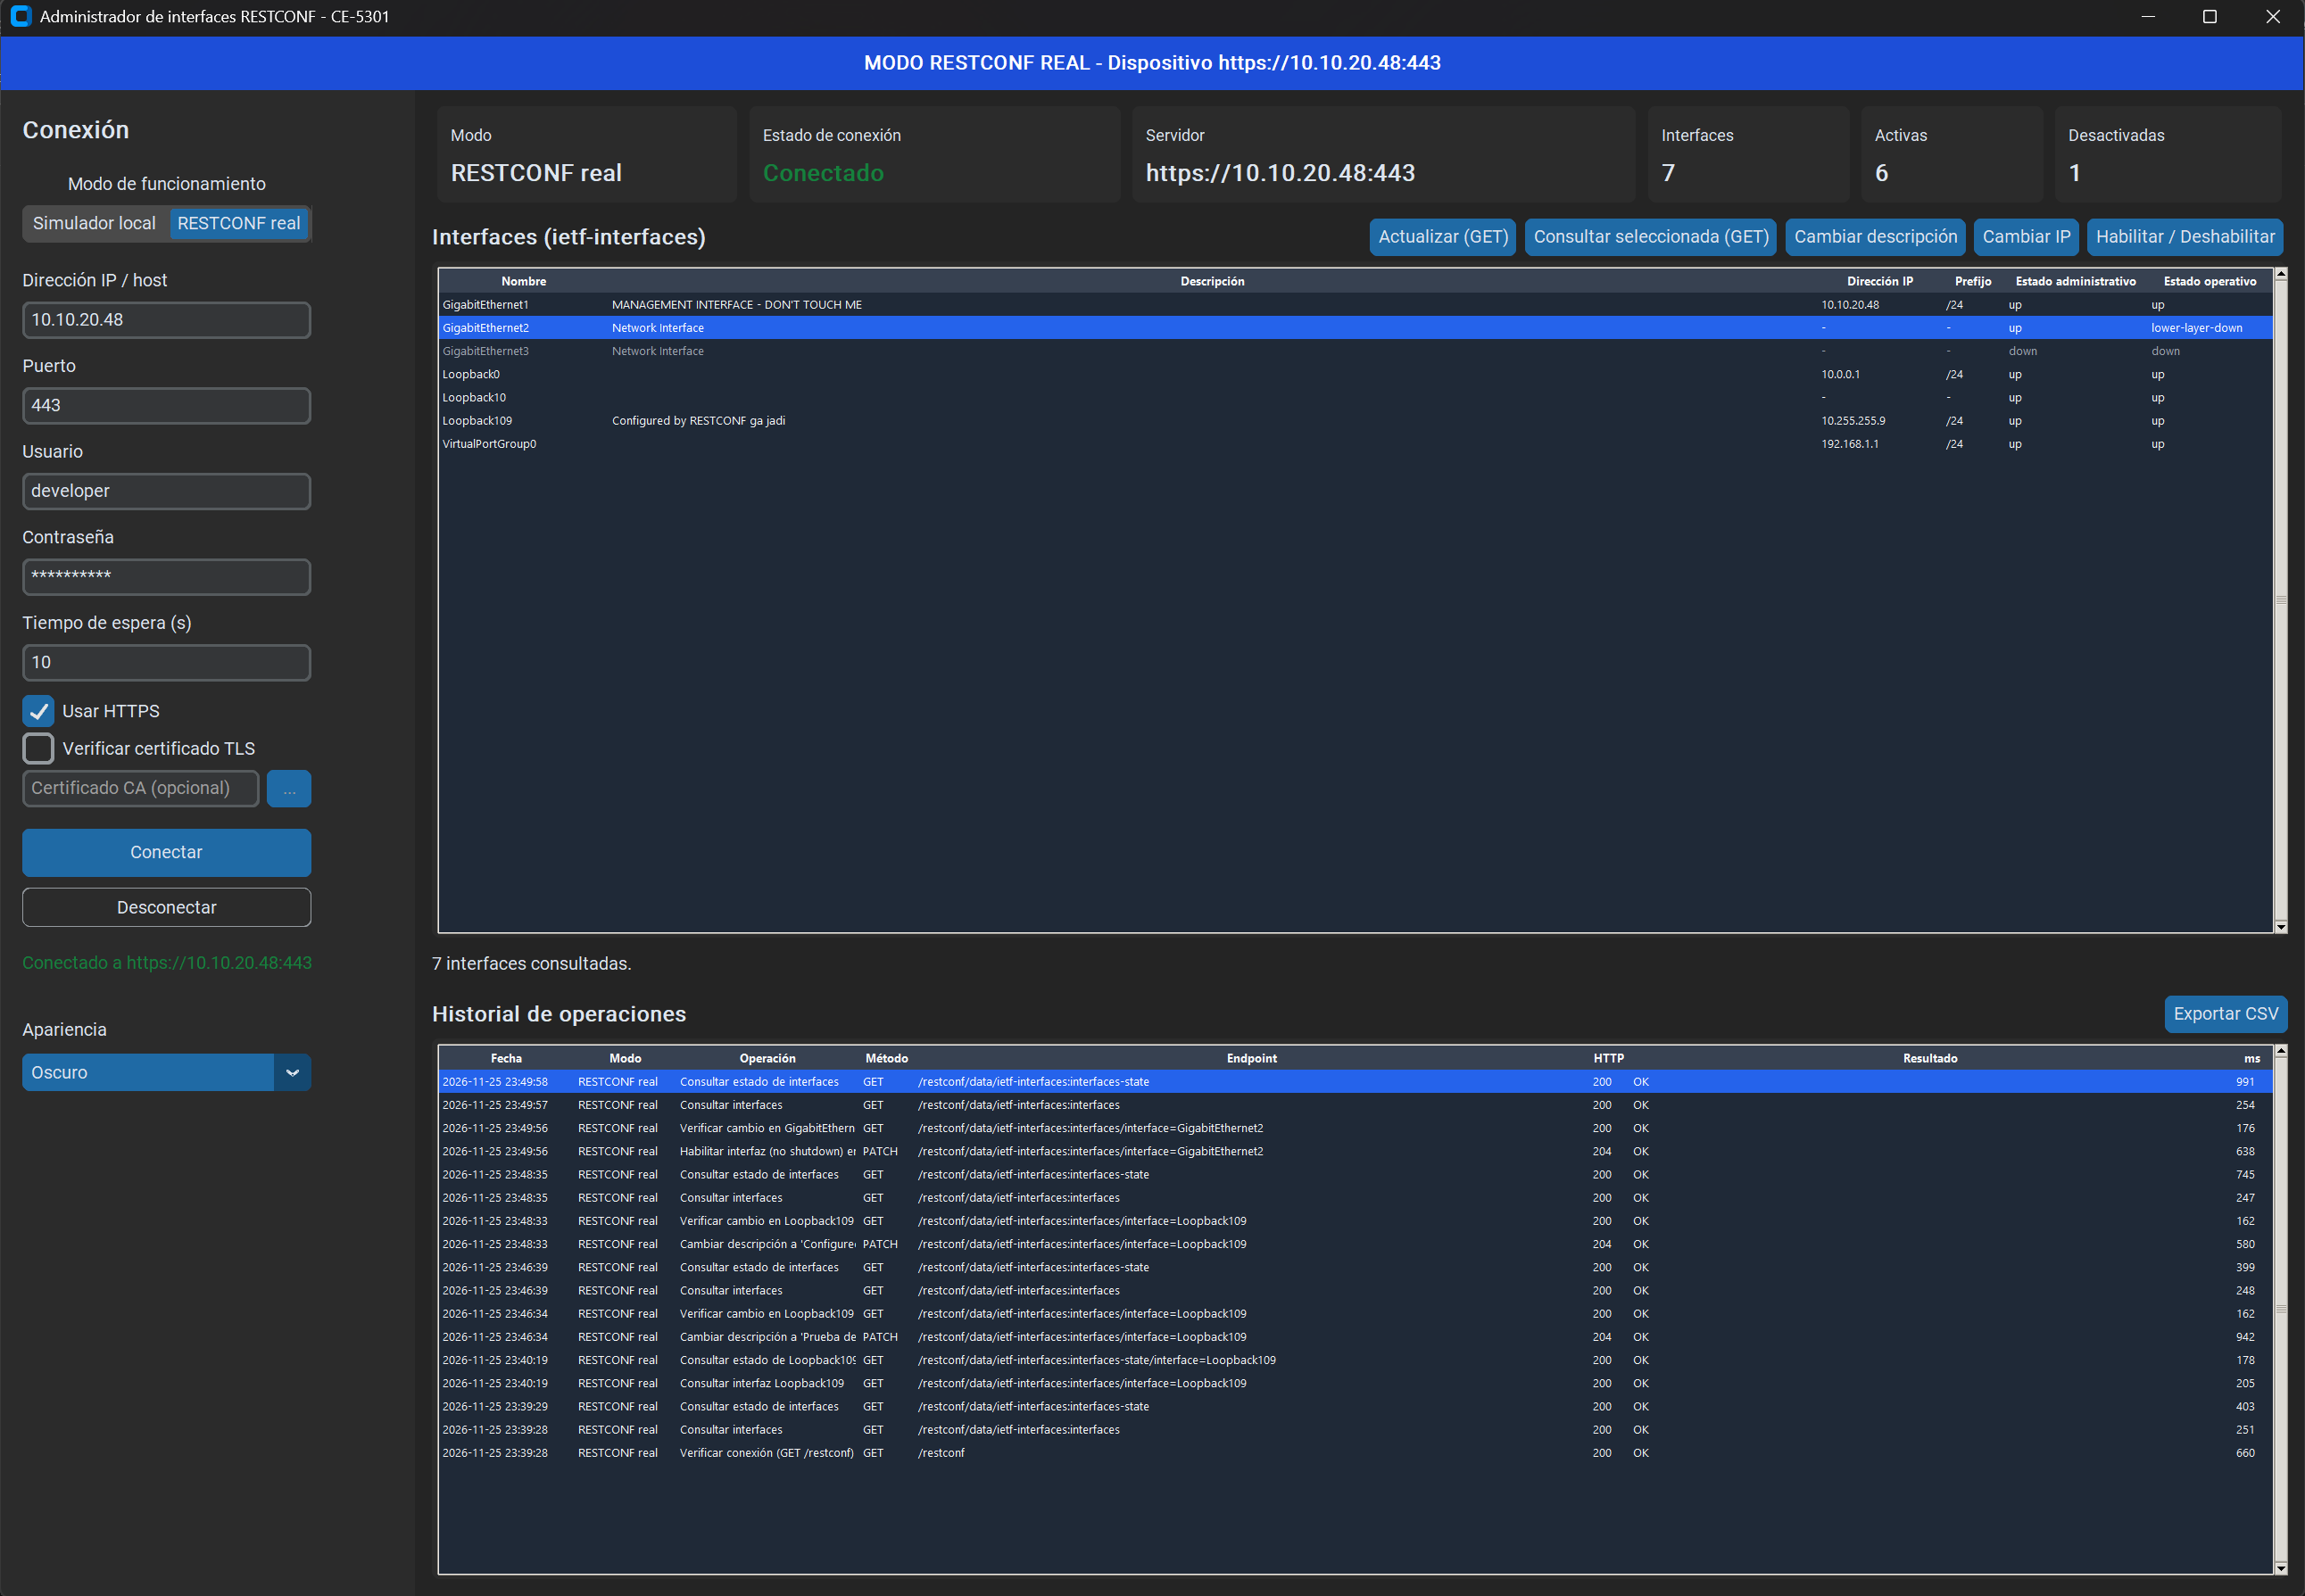
\includegraphics[width=0.95\textwidth]{cisco_GB_sim}
  \caption{GigabitEthernet2 habilitada: estado administrativo \texttt{up} y estado operativo \texttt{lower-layer-down} reportado por el router.}
  \label{fig:real_gi2}
\end{figure}

\subsection{Análisis cuantitativo}\label{sec:cuantitativo}
\textbf{Tiempos de respuesta.} Se midió cada operación 50 veces contra el simulador ejecutado en el mismo equipo (127.0.0.1), descartando una solicitud inicial de calentamiento. Los resultados se presentan en la Tabla~\ref{tab:tiempos}.

\begin{table}[H]
\centering
\caption{Tiempos de respuesta contra el simulador local (ms, $n=50$)}
\label{tab:tiempos}
\begin{tabular}{lrrrrr}
\toprule
\textbf{Operación} & \textbf{Promedio} & \textbf{Mediana} & \textbf{Desv. est.} & \textbf{P95} & \textbf{Máx.} \\
\midrule
GET interfaces & 2,07 & 2,03 & 0,37 & 2,69 & 3,18 \\
GET interfaz individual & 2,11 & 1,96 & 0,80 & 2,36 & 7,43 \\
PATCH descripción & 2,24 & 2,27 & 0,40 & 2,81 & 3,38 \\
PATCH + GET de verificación & 4,41 & 4,45 & 0,51 & 5,09 & 5,57 \\
\bottomrule
\end{tabular}
\end{table}

Las tres solicitudes individuales tienen tiempos similares, alrededor de 2~ms, y el cambio completo con verificación tarda aproximadamente el doble porque implica dos solicitudes. El máximo de 7,43~ms en el GET individual es un valor aislado: su mediana es 1,96~ms y su percentil 95 es 2,36~ms. Estos valores \textbf{no representan el tiempo de un router real}, en el que influyen la latencia de la red, el establecimiento de TLS y el procesamiento del dispositivo; solo muestran que el costo de la verificación posterior es una solicitud adicional.

\textbf{Comparación con el router real.} Contra el Catalyst 8000v, las consultas GET tardaron entre 162 y 403~ms, y los PATCH entre 580 y 942~ms (Tabla~\ref{tab:api_real}). Esto es unas dos órdenes de magnitud más que en el simulador, donde las solicitudes toman alrededor de 2~ms. La diferencia se explica por tres factores: el viaje de ida y vuelta a través de la VPN hasta el centro de datos de Cisco, el cifrado TLS y el procesamiento del propio IOS XE. La primera solicitud (660~ms) fue más lenta porque incluye el establecimiento de la sesión TLS. Las escrituras son las más costosas porque el dispositivo valida el cambio contra el modelo y lo aplica a la configuración en ejecución. Un cambio completo con su verificación tomó entre 742 y 1104~ms, un tiempo todavía adecuado para una operación interactiva. A diferencia de la Tabla~\ref{tab:tiempos}, estos valores son ejecuciones únicas y no un promedio estadístico.

\textbf{Entradas frente a salidas.} Para cambiar la descripción de una interfaz por CLI se requieren cinco comandos (\texttt{enable}, \texttt{configure terminal}, \texttt{interface}, \texttt{description} y \texttt{end}), más un \texttt{show} para verificar el resultado de forma visual. Con la aplicación, la misma operación es una sola solicitud PATCH seguida de un GET de verificación automático, cuyo resultado se compara con lo esperado y queda registrado con fecha, código HTTP y tiempo. De las 13 solicitudes de la Tabla~\ref{tab:api}, las 6 válidas (escenarios 1 a 5 y 13) fueron aceptadas, y las 6 que contenían un error del cliente o del recurso (escenarios 6 a 11) fueron rechazadas con el código esperado: 404, 401, 400, 400, 403 y 405. El escenario 12 corresponde a un error 500 provocado deliberadamente en el simulador para comprobar su manejo.

\subsection{Limitaciones encontradas}\label{sec:limitaciones}
\textbf{Ausencia de RESTCONF en el entorno de laboratorio.} El laboratorio se desarrolló en Cisco Packet Tracer 9.0.1. Para determinar si algún router del simulador permitía habilitar interfaces programables, se colocaron un router ISR4331 y un router 2901 y se ejecutaron, en modo de configuración global, los comandos \texttt{restconf}, \texttt{netconf-yang}, \texttt{ip http secure-server} e \texttt{ip http server}. En ambos equipos el simulador rechazó los cuatro comandos con el mensaje \texttt{\% Invalid input detected}. La prueba se repitió en R1 de la topología final con el mismo resultado (Listado~\ref{lst:restconf}).

\begin{lstlisting}[language={},caption={Rechazo de los comandos de RESTCONF en el ISR4331 de Packet Tracer},label={lst:restconf}]
R1(config)#restconf
% Invalid input detected at '^' marker.
R1(config)#netconf-yang
% Invalid input detected at '^' marker.
R1(config)#ip http secure-server
% Invalid input detected at '^' marker.
R1(config)#ip http server
% Invalid input detected at '^' marker.
\end{lstlisting}

\begin{figure}[H]
  \centering
  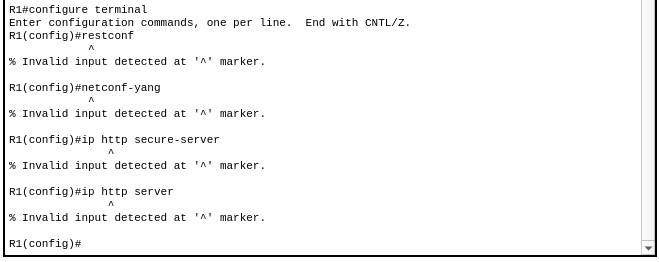
\includegraphics[width=\textwidth]{../../evidence/packet_tracer/restconf_rechazado_ISR4331.png}
  \caption{Rechazo de comandos de configuración RESTCONF y servicios HTTP/HTTPS en el router ISR4331 en Packet Tracer.}
  \label{fig:restconf_rechazado_ISR4331}
\end{figure}

\begin{figure}[H]
  \centering
  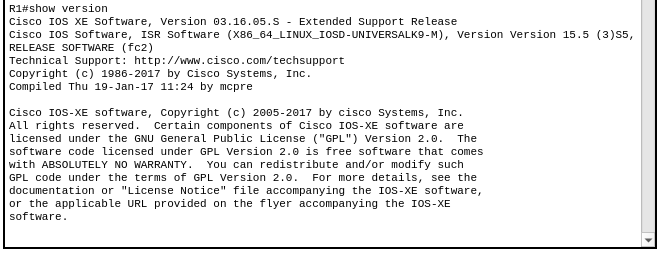
\includegraphics[width=\textwidth]{../../evidence/packet_tracer/show_version_ISR4331.png}
  \caption{Verificación de versión IOS (show version) en el router ISR4331 dentro de Packet Tracer.}
  \label{fig:show_version_ISR4331}
\end{figure}

\begin{figure}[H]
  \centering
  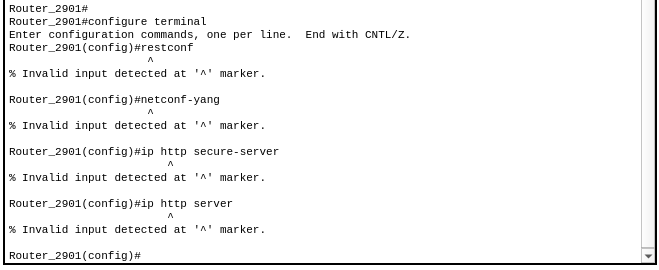
\includegraphics[width=\textwidth]{../../evidence/packet_tracer/restconf_rechazado_2901.png}
  \caption{. Comprobación del rechazo de comandos RESTCONF en router adicional (2901) en Packet Tracer.}
  \label{fig:restconf_rechazado_2901}
\end{figure}

Este resultado obedece al simulador y no al modelo de router seleccionado: según \texttt{show version}, el ISR4331 de Packet Tracer reporta Cisco IOS XE 16.6.4, y en equipos físicos Cisco documenta soporte de RESTCONF para la serie ISR 4000 a partir de IOS XE 16.3 \parencite{cisco_restconf}. Packet Tracer emula un subconjunto de comandos orientado a la enseñanza de configuración por CLI y no implementa el servidor HTTP de los routers, el agente RESTCONF ni los modelos YANG.

Se evaluó también el \textit{Network Controller} de Packet Tracer, que ofrece una API REST accesible desde el equipo anfitrión \parencite{pt_controller}. Se descartó porque esa API es propia del controlador, no sigue el RFC 8040 y no utiliza modelos YANG \parencite{rfc8040}.

El equipo no dispone de routers físicos compatibles. Por ello la solución se dividió en dos componentes independientes: el laboratorio de Packet Tracer, configurado y verificado mediante CLI, y la aplicación RESTCONF, probada contra un simulador local que sigue el modelo \texttt{ietf-interfaces} y el comportamiento HTTP del RFC 8040. La aplicación conserva un modo de conexión real, que finalmente se validó contra un router Catalyst 8000v virtual de Cisco DevNet Sandbox (Sección~\ref{sec:real}).
Este enfoque permitió avanzar en la validación de la aplicación RESTCONF sin depender de hardware físico.
No existe sincronización automática entre el simulador y Packet Tracer; la comparación entre ambos se realizó manualmente.

\textbf{Otras limitaciones.}
\begin{itemize}
  \item El simulador implementa un subconjunto del RFC 8040: no incluye POST, DELETE, codificación XML, parámetros de consulta, control de acceso NACM ni ETag. Admite una sola dirección IPv4 por interfaz y no permite crear interfaces.
  \item Los datos del simulador son ficticios, residen en memoria y se reinician al detenerlo.
  \item El simulador funciona por HTTP en el equipo local; un dispositivo real exige HTTPS y la validación de su certificado.
  \item Los tiempos medidos corresponden al equipo local y no son extrapolables a un router.
  \item Packet Tracer no acepta algunos comandos de IOS como \texttt{terminal length 0} ni \texttt{show running-config interface}, y el botón \textit{Copy} de su CLI no copia el texto, por lo que las salidas se transcribieron.
  \item En el router real se desactivó la verificación del certificado TLS, porque el sandbox utiliza un certificado autofirmado.
  \item El acceso al router real depende de una reserva temporal y de una VPN; las mediciones contra él son ejecuciones únicas y no un promedio estadístico.
\end{itemize}

% ----------------------------------------------------------------------
% CONCLUSIONES
% ----------------------------------------------------------------------
\section{Conclusiones y recomendaciones}

\subsection{Conclusiones}
\begin{enumerate}
  \item La programabilidad basada en modelos separa la estructura de los datos (YANG) del protocolo que los transporta (NETCONF o RESTCONF). Esta separación permitió que la misma aplicación funcione contra el simulador y contra un router IOS XE real sin cambiar su código.
  \item RESTCONF resultó adecuado para el caso de uso porque reutiliza HTTP, JSON y herramientas conocidas como Postman y \texttt{requests}. Las operaciones necesarias se resolvieron con GET, PATCH y PUT, y los errores con los códigos HTTP del RFC 8040.
  \item La elección entre PATCH y PUT depende del modelo: PATCH es apropiado para hojas simples como la descripción, mientras que para la dirección IP, cuya clave de lista es la propia dirección, fue necesario reemplazar la entrada completa con PUT.
  \item El laboratorio cumplió su objetivo: los tres routers convergieron con OSPF y se verificó la conectividad extremo a extremo entre las dos LAN. Sin embargo, se comprobó que Packet Tracer no implementa RESTCONF, por lo que no puede usarse como dispositivo administrado por la aplicación.
  \item Los objetivos del caso de uso se cumplieron tanto en el simulador como en un router Catalyst 8000v real con IOS XE 17.12.02: la aplicación consultó interfaces, validó y confirmó los cambios, los verificó con un GET posterior, manejó los errores definidos y registró las operaciones sin credenciales. Las cinco pruebas contra el dispositivo real se aprobaron sin modificar el código.
  \item Confirmar cada cambio antes de enviarlo y verificarlo después tiene un costo pequeño (una solicitud adicional) y aporta trazabilidad, a diferencia de la verificación visual por CLI.
  \item El dispositivo real permitió observar la diferencia entre configuración y estado que define el modelo YANG: una interfaz habilitada (\texttt{enabled} igual a \texttt{true}) puede seguir sin operar (\texttt{lower-layer-down}). Por eso la verificación de un cambio debe considerar ambos datos.
\end{enumerate}

\subsection{Recomendaciones}
\begin{enumerate}
  \item Repetir las mediciones contra el router real con un número mayor de muestras y validar su certificado TLS mediante una autoridad de certificación de confianza, en lugar de desactivar la verificación.
  \item Para un laboratorio propio, usar imágenes virtuales de IOS XE (Catalyst 8000V) en emuladores como Cisco Modeling Labs o GNS3, en lugar de Packet Tracer.
  \item Extender la aplicación a varios dispositivos con un inventario y ejecutar las consultas en paralelo.
  \item Incorporar control de cambios: comparación de configuración antes y después, aprobación previa y reversión automática si la verificación falla.
  \item Usar NETCONF cuando se requieran transacciones con el datastore \textit{candidate} y confirmación en varios equipos.
  \item Reforzar la seguridad con HTTPS y validación de certificados, cuentas con privilegios mínimos y almacenamiento seguro de credenciales.
  \item Complementar con monitoreo continuo mediante telemetría basada en modelos o SNMP.
\end{enumerate}

% ----------------------------------------------------------------------
% REFERENCIAS
% ----------------------------------------------------------------------
\newpage
\printbibliography[title={Referencias bibliográficas}]

% ----------------------------------------------------------------------
% ANEXO 1
% ----------------------------------------------------------------------
\appendix
\section{Configuraciones y código fuente}

\subsection{Configuración de dispositivos Packet Tracer}
El Listado~\ref{lst:r1cfg} contiene la configuración aplicada a R1. Las de R2, R3, S1 y S2 siguen la misma estructura y se encuentran en \texttt{lab/configuraciones/} del repositorio \parencite{repositorio}.

\begin{lstlisting}[language={},caption={Configuración de R1},label={lst:r1cfg}]
hostname R1
no ip domain-lookup
enable secret class
banner motd #Laboratorio CE-5301 - Acceso solo autorizado#
interface GigabitEthernet0/0/0
 description Enlace WAN hacia R2
 ip address 10.0.12.1 255.255.255.252
 no shutdown
interface GigabitEthernet0/0/1
 description LAN1 - red de usuarios
 ip address 192.168.10.1 255.255.255.0
 no shutdown
interface GigabitEthernet0/0/2
 description Sin uso
 shutdown
interface Loopback0
 description Identificador del router (router-id OSPF)
 ip address 1.1.1.1 255.255.255.255
router ospf 1
 router-id 1.1.1.1
 network 10.0.12.0 0.0.0.3 area 0
 network 192.168.10.0 0.0.0.255 area 0
 network 1.1.1.1 0.0.0.0 area 0
 passive-interface GigabitEthernet0/0/1
line console 0
 logging synchronous
\end{lstlisting}

\begin{table}[H]
\centering
\caption{Diferencias de configuración de R2 y R3 respecto de R1}
\begin{tabularx}{\textwidth}{p{1.3cm}X}
\toprule
\textbf{Router} & \textbf{Cambios} \\
\midrule
R2 & G0/0/0 10.0.12.2/30, G0/0/1 10.0.23.1/30, Loopback0 2.2.2.2; redes OSPF 10.0.12.0/30, 10.0.23.0/30 y 2.2.2.2/32; sin interfaces pasivas \\
R3 & G0/0/0 10.0.23.2/30, G0/0/1 192.168.20.1/24, Loopback0 3.3.3.3; redes OSPF 10.0.23.0/30, 192.168.20.0/24 y 3.3.3.3/32; G0/0/1 pasiva \\
\bottomrule
\end{tabularx}
\end{table}

\subsection{Código fuente}
El código completo se encuentra en el repositorio \url{https://github.com/CAMF0712/Proyecto_Redes} \parencite{repositorio}. Su organización es la siguiente:
\begin{itemize}
  \item \texttt{main.py} y \texttt{application/}: aplicación gráfica y cliente RESTCONF.
  \item \texttt{simulator/}: simulador RESTCONF.
  \item \texttt{models/}: módulos YANG validados con pyang.
  \item \texttt{tests/}: pruebas automatizadas.
  \item \texttt{lab/}: topología \texttt{.pkt}, configuraciones y procedimientos de verificación.
  \item \texttt{evidence/}: evidencias del simulador, del laboratorio, de las pruebas y de pyang.
  \item \texttt{docs/}: arquitectura, guía para dispositivo real, limitaciones, guion y este informe.
\end{itemize}
El repositorio no contiene contraseñas de dispositivos reales; las únicas credenciales incluidas son las de prueba del simulador local.

\subsection{Colección Postman}
La colección se encuentra en \path{postman/collection.json}, con los entornos \path{entorno_simulador.json} y \path{entorno_dispositivo_real.json}. Incluye GET de interfaces, GET de una interfaz, PATCH de la descripción, GET de verificación y tres casos de error (404, 401 y 400), con autenticación básica, encabezados, cuerpos JSON, pruebas automáticas y ejemplos de respuesta generados con el simulador.

% ----------------------------------------------------------------------
% ANEXO 2: TRABAJO INDIVIDUAL Y EN EQUIPO
% ----------------------------------------------------------------------
\section{Trabajo individual y en equipo}

\subsection{Metas del proyecto y entregables}
\begin{itemize}
  \item Informe técnico con investigación, caso de uso, resultados y referencias.
  \item Aplicación de administración de interfaces, simulador y pruebas automatizadas.
  \item Topología de Packet Tracer, configuraciones y evidencias del laboratorio.
  \item Colección Postman y código fuente en el repositorio.
  \item Video de demostración de máximo diez minutos.
  \item Minutas, cronograma y bitácoras individuales.
\end{itemize}

\subsection{Roles y responsabilidades}
\begin{longtable}{p{3.6cm}p{3.4cm}p{6.6cm}}
\caption{Distribución de roles del equipo}\\
\toprule
\textbf{Integrante} & \textbf{Rol} & \textbf{Responsabilidades} \\
\midrule
\endfirsthead
\toprule
\textbf{Integrante} & \textbf{Rol} & \textbf{Responsabilidades} \\
\midrule
\endhead
Giancarlo Vega Marín (2020195338) & Coordinador del proyecto y del informe & Planificar el trabajo, coordinar reuniones y minutas, integrar el informe, revisar la investigación teórica y la bibliografía \\
José Manuel Loría Cordero (2022211671) & Responsable del laboratorio de red & Diseñar la topología y el direccionamiento, configurar los equipos en Packet Tracer, verificar OSPF y conectividad, capturar evidencias del laboratorio \\
César Andrés Mora Fajardo (2020053458) & Desarrollador de la aplicación & Implementar el cliente RESTCONF, la lógica de administración de interfaces y la interfaz gráfica; mantener el repositorio \\
Marco Villatoro Chacon (2021057692) & Desarrollador del simulador y modelos YANG & Implementar el simulador RESTCONF, validar los modelos YANG con pyang, documentar el uso con un dispositivo real \\
Mariana Rojas Rojas (2020076936) & Responsable de pruebas y evidencias & Diseñar y ejecutar las pruebas automatizadas, preparar la colección Postman, generar evidencias y coordinar el video \\
\bottomrule
\end{longtable}

\subsection{Reglas de trabajo}
\begin{enumerate}
  \item Mantener comunicación periódica y documentar acuerdos.
  \item Cumplir las responsabilidades y fechas acordadas.
  \item Compartir avances verificables y avisar oportunamente sobre bloqueos.
  \item Revisar en equipo los cambios importantes del código y de la configuración.
  \item Mantener respaldos y control de versiones de los entregables.
  \item No compartir credenciales ni datos sensibles en repositorios o documentos públicos.
\end{enumerate}

\subsection{Cronograma}
\begin{longtable}{p{4.0cm}p{3.2cm}p{2.7cm}p{3.7cm}}
\caption{Cronograma de actividades}\\
\toprule
\textbf{Actividad} & \textbf{Responsable} & \textbf{Fecha} & \textbf{Estado / evidencia} \\
\midrule
\endfirsthead
\toprule
\textbf{Actividad} & \textbf{Responsable} & \textbf{Fecha} & \textbf{Estado / evidencia} \\
\midrule
\endhead
Investigación bibliográfica & Giancarlo Vega & 25/11/2026 & Completada; Sección 2 \\
Diseño y configuración de la topología & José Manuel Loría & 25/11/2026 & Completada; \texttt{lab/} \\
Prueba de RESTCONF en Packet Tracer & José Manuel Loría & 25/11/2026 & Completada; carpeta \texttt{lab/} \\
Modelos YANG y simulador & Marco Villatoro & 25/11/2026 & Completada; \texttt{models/} y \texttt{simulator/} \\
Validación en router real (DevNet Sandbox) & Marco Villatoro & 25/11/2026 & Completada; Sección~\ref{sec:real} \\
Desarrollo de la aplicación & César Mora & 25/11/2026 & Completada; \texttt{application/} \\
Pruebas, Postman y evidencias & Mariana Rojas & 25/11/2026 & Completada; \texttt{tests/}, \texttt{postman/} y \texttt{evidence/} \\
Revisión final del informe & Giancarlo Vega & \pendiente{fecha} & En curso \\
Grabación del video & Mariana Rojas & \pendiente{fecha} & Pendiente \\
\bottomrule
\end{longtable}

\subsection{Minutas de reuniones}
\vspace{0.4cm}

\textbf{Reunión 1 -- Coordinación de cierre del proyecto}\par
Fecha: 25 de noviembre de 2026\\
Participantes: Giancarlo, José, César, Marco, Mariana\\
Temas tratados:
\begin{itemize}
    \item Organización del equipo para completar los entregables pendientes
    antes de la fecha de entrega.
    \item Revisión de las tareas pendientes identificadas en la guía del equipo.
    \item Coordinación de la revisión final del informe, evidencias y video de demostración.
    \item Distribución y seguimiento de las responsabilidades asignadas a cada integrante.
\end{itemize}

Acuerdos y responsables:
\begin{itemize}
    \item \textbf{Giancarlo Vega Marín:} coordinación del cierre, revisión y
    compilación del informe final.
    \item \textbf{José Manuel Loría Cordero:} completar y recopilar las
    evidencias pendientes del laboratorio de Packet Tracer.
    \item \textbf{César Andrés Mora Fajardo:} completar las evidencias de la
    aplicación y la tabla de comparación entre CLI y aplicación.
    \item \textbf{Marco Villatoro Chacón:} preparar y completar los
    entregables correspondientes al simulador y los modelos YANG.
    \item \textbf{Mariana Rojas Rojas:} completar las evidencias de pruebas,
    Postman y coordinar la grabación del video de demostración.
    \item Todos los integrantes: completar sus bitácoras individuales,
    participar en el video y realizar la autoevaluación y coevaluación.
\end{itemize}

\vspace{0.4cm}

\textbf{Reuniones adicionales}\par
\pendiente{Registrar únicamente si se realizan reuniones adicionales antes de la entrega.}

\subsection{Bitácora individual}

La siguiente tabla resume las actividades de finalización, revisión,
integración y preparación de los entregables del proyecto.

\begin{longtable}{p{3.4cm}p{2.0cm}p{1.4cm}p{6.6cm}}
\caption{Bitácora de actividades del equipo} \\
\toprule
\textbf{Integrante} & \textbf{Fecha} & \textbf{Horas} &
\textbf{Actividad} \\
\midrule
\endfirsthead

\toprule
\textbf{Integrante} & \textbf{Fecha} & \textbf{Horas} &
\textbf{Actividad} \\
\midrule
\endhead

Giancarlo Vega Marín &
25/11/2026 & 5 &
Coordinación del equipo, revisión de la estructura y contenido del informe,
organización de los entregables y preparación del documento en LaTeX. \\

Giancarlo Vega Marín &
26/11/2026 & 4 &
Revisión final del informe, corrección de formato y referencias, integración
de pendientes, compilación del PDF definitivo y verificación de la entrega. \\

José Manuel Loría Cordero &
25/11/2026 & 4 &
Revisión del laboratorio de Packet Tracer, verificación de la topología,
configuración de routers, OSPF y conectividad entre los equipos. \\

José Manuel Loría Cordero &
26/11/2026 & 3 &
Recopilación y organización de evidencias del laboratorio, revisión de
comandos de verificación y preparación de resultados para el informe y video. \\

César Andrés Mora Fajardo &
25/11/2026 & 5 &
Revisión de la aplicación en Python, verificación de las funcionalidades
RESTCONF, operaciones sobre interfaces y flujo de confirmación y verificación
de cambios. \\

César Andrés Mora Fajardo &
26/11/2026 & 3 &
Pruebas finales de la aplicación, revisión de resultados, preparación de
capturas de la interfaz y documentación de la comparación entre CLI y aplicación. \\

Marco Villatoro Chacón &
25/11/2026 & 3 &
Estudio de la especificación y del repositorio; ejecución del simulador y
de la aplicación; exploración de los modelos YANG con pyang; pruebas GET,
PATCH y de errores (400 y 403) con curl; reserva del sandbox Catalyst 8000v,
configuración de la VPN y validación del modo real (5/5 pruebas aprobadas y
operaciones con la aplicación). \\

Marco Villatoro Chacón &
26/11/2026 & 3 &
Revisión final del simulador y modelos YANG, preparación de la explicación
técnica de su funcionamiento y organización de su participación en el video. \\

Mariana Rojas Rojas &
25/11/2026 & 4 &
Ejecución y revisión de las pruebas automatizadas, organización de resultados
de pytest y preparación de las pruebas de API mediante Postman. \\

Mariana Rojas Rojas &
26/11/2026 & 4 &
Verificación de las pruebas finales, organización de evidencias, coordinación
de la grabación del video de demostración y revisión de los entregables. \\

\bottomrule
\end{longtable}


\subsection{Evaluación de la eficiencia del trabajo en equipo}
Cada integrante debe realizar una autoevaluación y una coevaluación honesta y fundamentada sobre su desempeño y el de sus compañeros. Además, la consigna establece completar el formulario individual indicado por el profesor. El formulario debe ser completado por cada estudiante una sola vez:

\url{https://docs.google.com/forms/d/e/1FAIpQLSfC_crNLh92D2pbcmpS1f_qeWVgdBkoXvHkjbXpWi53Q9b6UQ/viewform}

\begin{figure}[H]
	\centering
	
\includegraphics[width=\textwidth]{../../evidence/evaluacion/evaluacion_cesar.jpg}
	\caption{. Evidencia - César.}
	\label{fig:evaluacion_cesar}
\end{figure}


\begin{figure}[H]
	\centering
	
\includegraphics[width=\textwidth]{../../evidence/evaluacion/evaluacion_gvm.jpg}
	\caption{. Evidencia - Giancarlo.}
	\label{fig:evaluacion_gvm}
\end{figure}

\begin{figure}[H]
	\centering
	
\includegraphics[width=0.55\textwidth]{../../evidence/evaluacion/evaluacion_mariana.jpg}
	\caption{. Evidencia - Mariana.}
	\label{fig:evaluacion_mariana}
\end{figure}

\begin{figure}[H]
	\centering
	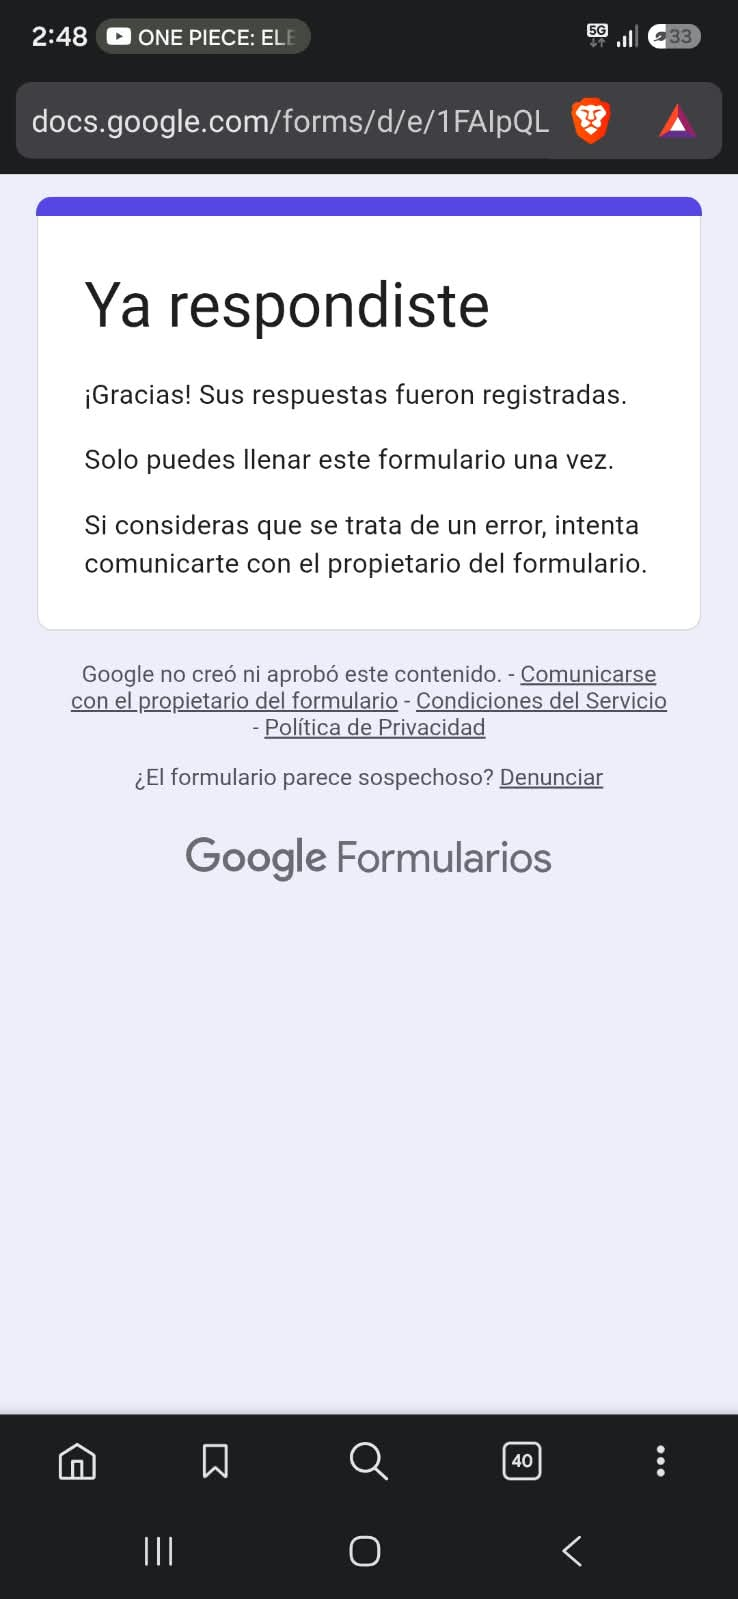
\includegraphics[width=0.55\textwidth]{../../evidence/evaluacion/evaluacion_jose.jpg}
	\caption{. Evidencia - Jose.}
	\label{fig:evaluacion_jose}
\end{figure}

\begin{figure}[H]
	\centering
	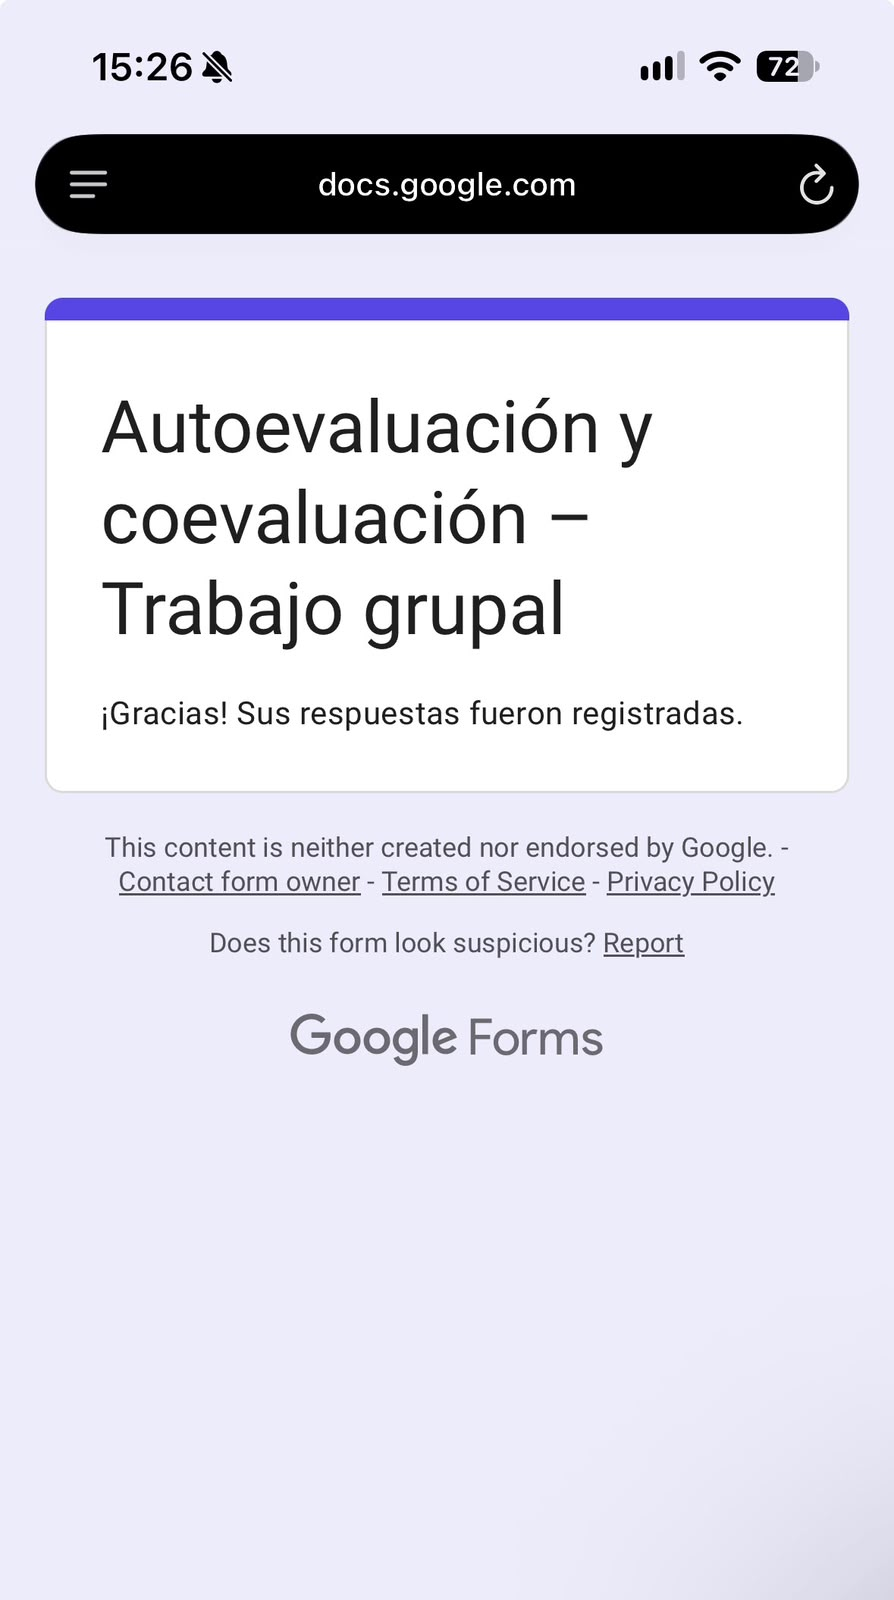
\includegraphics[width=0.55\textwidth]{../../evidence/evaluacion/evaluacion_marco.jpg}
	\caption{. Evidencia - Marco.}
	\label{fig:evaluacion_marco}
\end{figure}



\end{document}
